
\documentclass{beamer}
\usecolortheme{dove}
\setbeamertemplate{navigation symbols}{}
\setbeamertemplate{footline}[text line]{\parbox{\linewidth}{\vspace*{-8pt}\insertsectionnavigationhorizontal{.97\paperwidth}{\hspace{-32pt}}{\hfill\hfill}}}
\usepackage{amsmath,amssymb,amsfonts,amsthm, multicol, subfigure, color}
\usepackage{bm}
\usepackage{graphicx}
\usepackage{tabularx}
\usepackage{booktabs}
\usepackage{hyperref}
\usepackage{pdfpages}
\usepackage{xcolor}
\definecolor{seagreen}{RGB}{46, 139, 87}
\definecolor{ucla}{RGB}{39, 116, 174}
\definecolor{darkestblue}{RGB}{0, 59, 92}
\definecolor{gold}{RGB}{255, 209, 0}
\def\independenT#1#2{\mathrel{\rlap{$#1#2$}\mkern2mu{#1#2}}}
\newcommand\indep{\protect\mathpalette{\protect\independenT}{\perp}}
\def\log{\text{log}}
\newcommand\logit{\text{logit}}
\newcommand\iid{\stackrel{\text{iid}}{\sim}}
\newcommand\E{\text{E}}
\newcommand\V{\text{V}}
\renewcommand\P{\text{P}}
\newcommand{\Cov}{\text{Cov}}
\newcommand{\Cor}{\text{Cor}}
\newcommand\doop{\text{do}}
\usepackage{stackrel}
\usepackage{tikz}
\usetikzlibrary{arrows,shapes.arrows,positioning,shapes,patterns,calc}
\newcommand\slideref[1]{\vskip .1cm \tiny \textcolor{gray}{{#1}}}
\newcommand\red[1]{\color{red}#1}
\newcommand\blue[1]{\color{blue}#1}
\newcommand\gray[1]{\color{gray}#1}
\newcommand\seagreen[1]{\color{seagreen}#1}
\newcommand\purple[1]{\color{purple}#1}
\newcommand\orange[1]{\color{orange}#1}
\newcommand\black[1]{\color{black}#1}
\newcommand\white[1]{\color{white}#1}
\newcommand\teal[1]{\color{teal}#1}
\newcommand\magenta[1]{\color{magenta}#1}
\newcommand\Fuchsia[1]{\color{Fuchsia}#1}
\newcommand\BlueGreen[1]{\color{BlueGreen}#1}
\newcommand\bblue[1]{\textcolor{blue}{\textbf{#1}}}
\newcommand\bred[1]{\textcolor{red}{\textbf{#1}}}
\newcommand\bgray[1]{\textcolor{gray}{\textbf{#1}}}
\newcommand\bgreen[1]{\textcolor{seagreen}{\textbf{#1}}}
\newcommand\bref[2]{\href{#1}{\color{blue}{#2}}}
\colorlet{lightgray}{gray!40}
\pgfdeclarelayer{bg}    % declare background layer for tikz
\pgfsetlayers{bg,main} % order layers for tikz
\newcommand\mycite[1]{\begin{scriptsize}\textcolor{darkgray}{(#1)}\end{scriptsize}}
\newcommand{\tcframe}{\frame{
%\small{
\only<1|handout:0>{\tableofcontents}
\only<2|handout:1>{\tableofcontents[currentsubsection]}}
%}
}
\usepackage{soul}

\usepackage[round]{natbib}
\bibliographystyle{humannat-mod}
\setbeamertemplate{enumerate items}[default]
\usepackage{mathtools}

\newcommand{\goalsframe}{\begin{frame}{Learning goals for today}
By the end of class, you will be able to
\begin{itemize}
    \item define causal effects
    \item identify average causal effects by
    \begin{itemize}
    \item exchangeability
    \item conditional exchangeability
    \end{itemize}
    \item select a sufficient adjustment set using a Directed Acyclic Graph
\end{itemize} \vskip .2in
\end{frame}}

\title{Nonparametric Causal Identification}
\author{UCLA SOCIOL 212B\\Winter 2025}
\date{19 Feb 2025}

\begin{document}

\maketitle

\goalsframe

\section{Define Causal Effects}

\begin{frame}{Causal claims hinge on arguments, not on data}

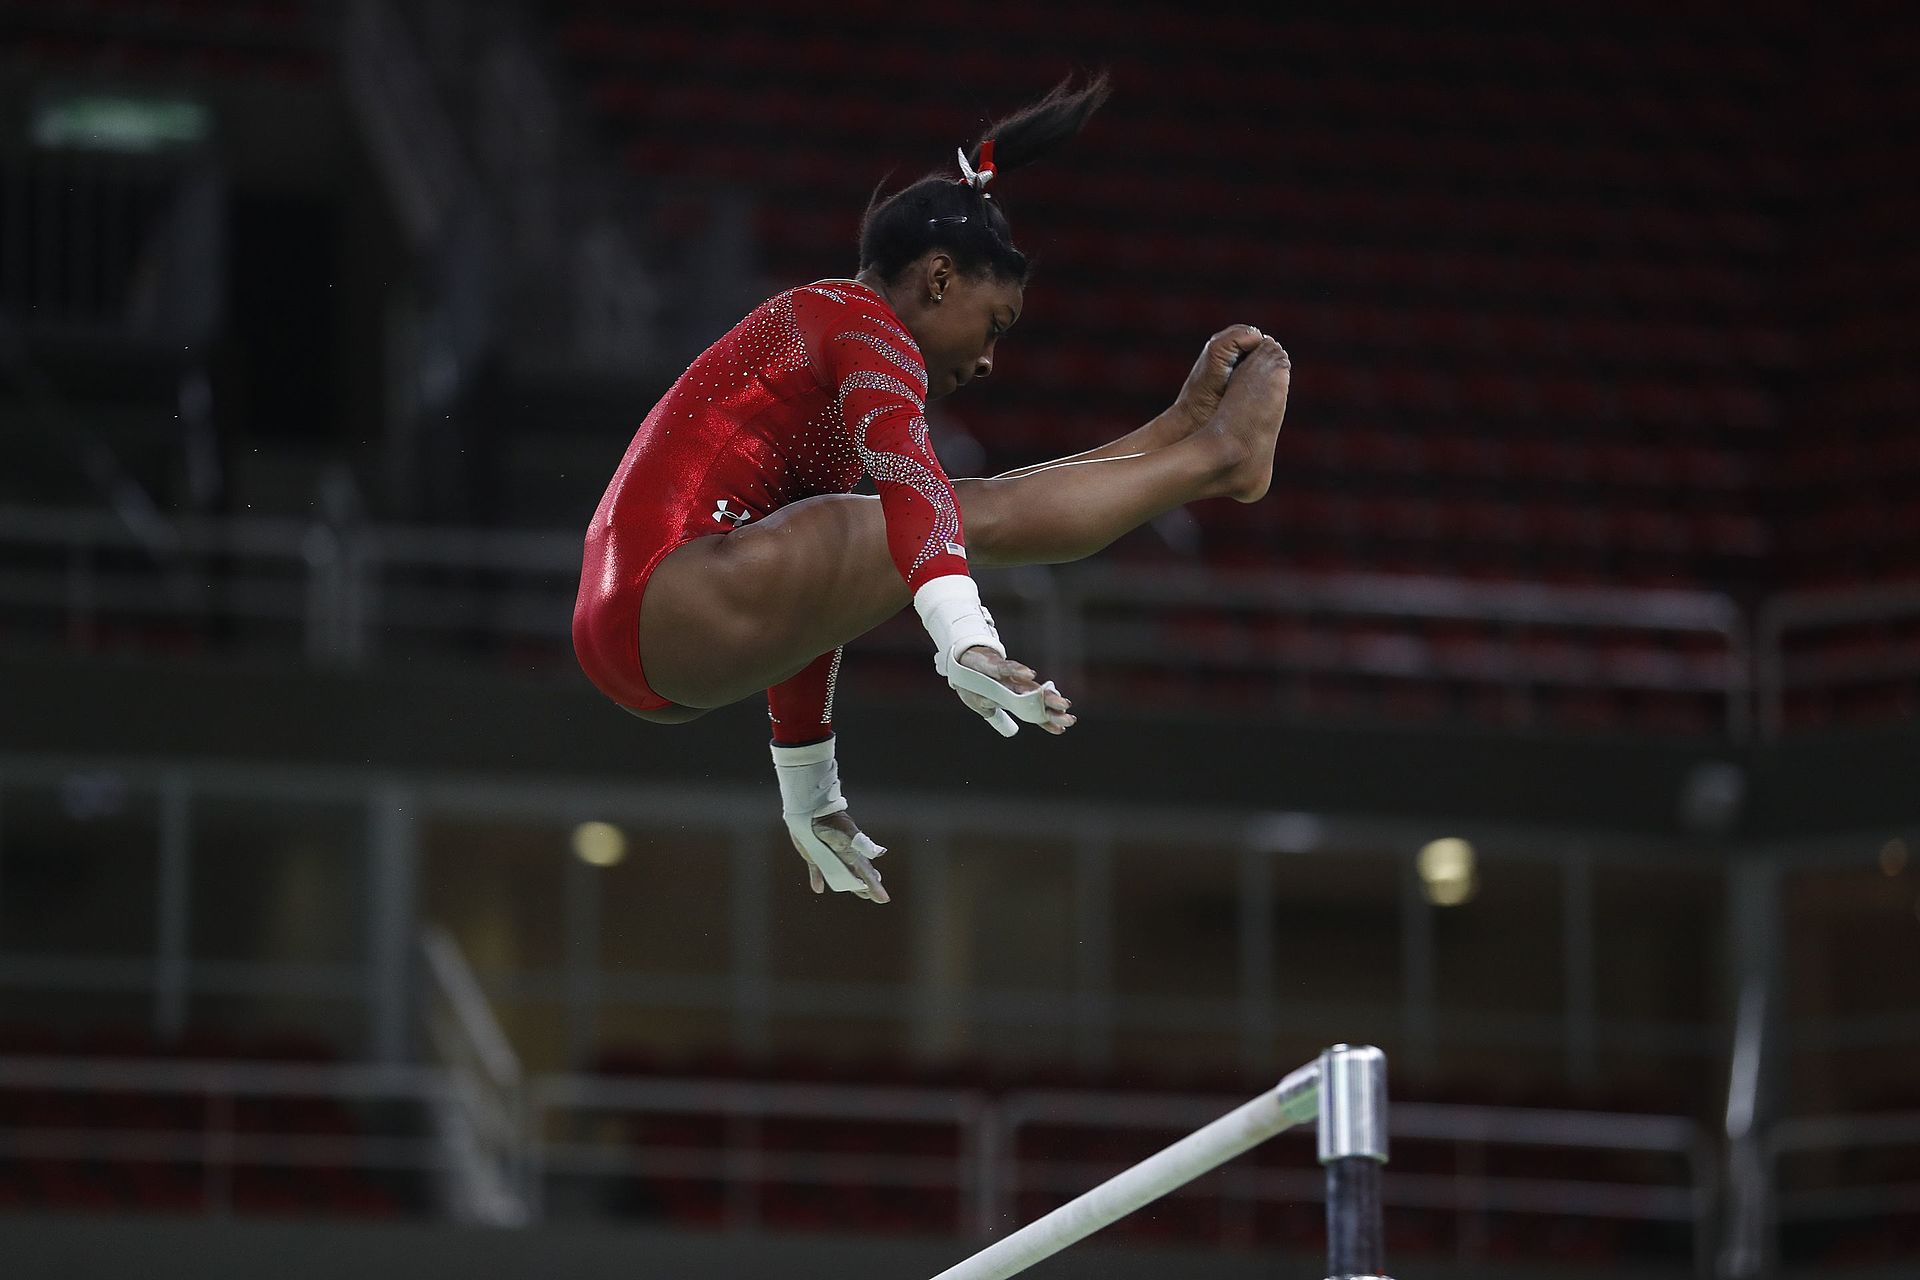
\includegraphics[width = .6\textwidth]{figures/Biles_bar}
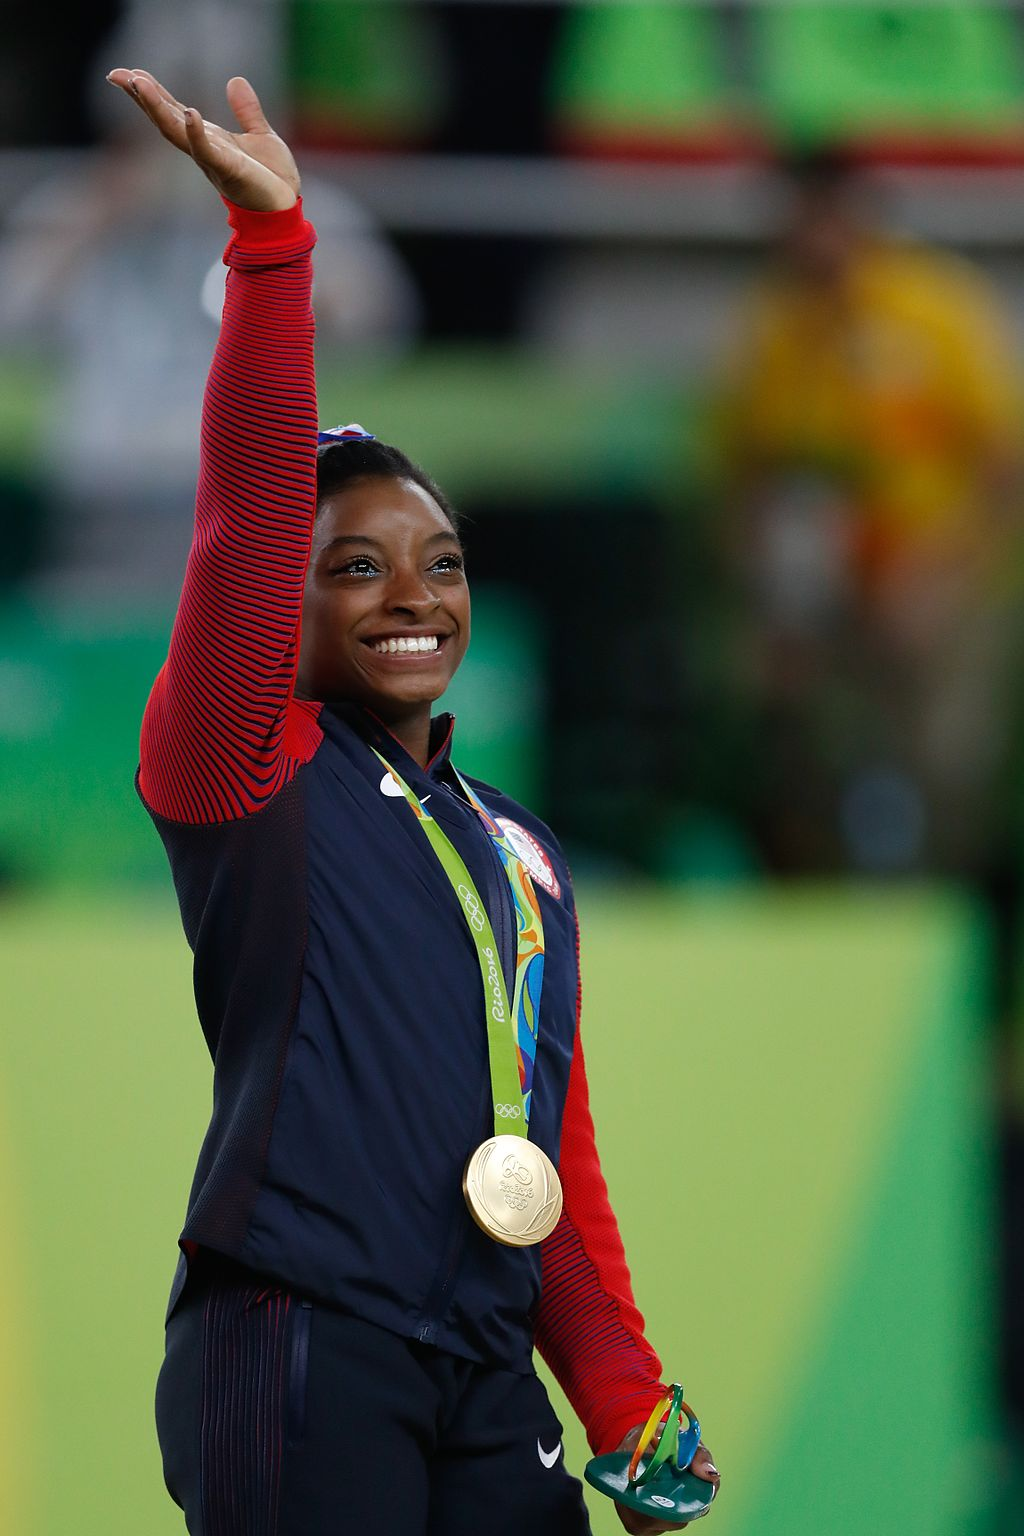
\includegraphics[width = .3\textwidth]{figures/Biles_medal}

\vskip .2in
\begin{tiny}
Left photo: By Fernando Frazão/Agência Brasil - \url{http://agenciabrasil.ebc.com.br/sites/_agenciabrasil2013/files/fotos/1035034-_mg_0802_04.08.16.jpg, CC BY 3.0 br, https://commons.wikimedia.org/w/index.php?curid=50548410} \\
Right photo: By Agencia Brasil Fotografias - EUA levam ouro na ginástica artística feminina; Brasil fica em 8 lugar, CC BY 2.0, \url{https://commons.wikimedia.org/w/index.php?curid=50584648}\\
\end{tiny}

\end{frame}

\begin{frame}{Causal claims hinge on arguments, not on data}
\begin{enumerate}
\item Statistical evidence
\begin{itemize}
\item Simone Biles swung on the uneven bars. She won a gold medal. \pause
\item I did not swing on the uneven bars. I did not win a gold medal.
\end{itemize} \pause
\item Possible causal claim
\begin{itemize}
\item Swinging on the uneven bars causes a person to win a gold medal.
\end{itemize}
\end{enumerate} \vskip .2in \pause
\begin{tabular}{rccc}
& \multicolumn{2}{l}{Do you win gold if you:} & Causal effect \\
& Swing & Do not swing & of swinging \\
\hline
Simone Biles & Yes (1) & \only<1-4>{?}\only<5->{\blue{No (0)}} & \only<1-5>{?}\only<6->{+1} \\
Ian & \only<1-6>{?}\only<7->{\blue{No (0)}} & No (0) & \only<1-7>{?}\only<8->{0} \\
\hline
\end{tabular}
\end{frame}

\begin{frame}
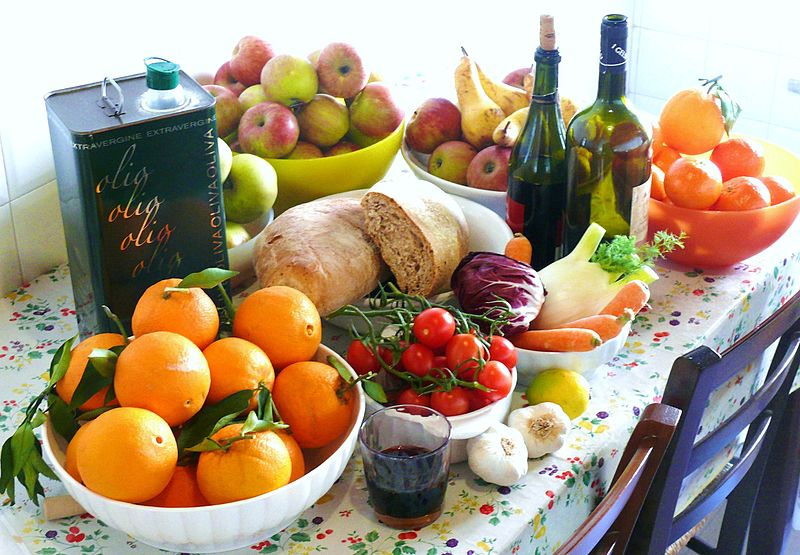
\includegraphics[width = \textwidth]{figures/mediterranean_diet}
\end{frame}

\begin{frame}{Fundamental problem of causal inference}{\href{https://www.tandfonline.com/doi/abs/10.1080/01621459.1986.10478354}{Holland 1986}}

\begin{tikzpicture}[x = \textwidth, y = .8\textheight]
\node at (0,0) {};
\node at (1,1) {};
% Factual outcomes
\node[anchor = north, align = center] at (.25,1) {Descriptive evidence};
\foreach \i in {1,...,8} {
	\node[font = \tiny, anchor = west] at (-.05,9/20-\i/20 + .175) {Person \i};
}
\foreach \i in {.2,.3,.35,.45,.55} {
	\draw[fill = blue, opacity = .3, color = blue] (.05,\i) rectangle (.25,\i + .05) {};
	\node[font = \tiny] at (.15,\i + .025) {lifespan};
}
\foreach \i in {.25,.4,.5} {
	\draw[fill = seagreen, opacity = .3, color = seagreen] (.25,\i) rectangle (.45,\i + .05) {};
	\node[font = \tiny] at (.35,\i + .025) {lifespan};
}
\node[font = \footnotesize, align = center, fill = blue, fill opacity = .3, text opacity = 1] at (.15,.8) {average\\lifespan};
\node[font = \footnotesize, align = center, fill = seagreen, fill opacity = .3, text opacity = 1] at (.35,.8) {average\\lifespan};
\node at (.25,.8) {$-$};
%\node[font = \tiny] at (.15,.575) {$Y_1^\text{Mediterranean Diet}$};
%\node[font = \tiny] at (.35,.525) {$Y_2^\text{Standard Diet}$};
%\node[font = \tiny] at (.15,.475) {$Y_3^\text{Mediterranean Diet}$};
%\node[font = \tiny] at (.35,.425) {$Y_4^\text{Standard Diet}$};
%\node[font = \tiny] at (.15,.375) {$Y_5^\text{Mediterranean Diet}$};
%\node[font = \tiny] at (.15,.325) {$Y_6^\text{Mediterranean Diet}$};
%\node[font = \tiny] at (.35,.275) {$Y_7^\text{Standard Diet}$};
%\node[font = \tiny] at (.15,.225) {$Y_8^\text{Mediterranean Diet}$};
\node[anchor = north, align = center, font = \footnotesize, blue] at (.15, .2) {Outcome\\under\\Mediterranean\\diet};
\node[anchor = north, align = center, font = \footnotesize, seagreen] at (.35, .2) {Outcome\\under\\standard\\diet};
\pause
% Potential outcomes
\node[anchor = north, align = center] at (.75,1) {Causal claim};
\node[font = \footnotesize, align = center, fill = blue, fill opacity = .3, text opacity = 1] at (.65,.8) {average\\lifespan};
\node[font = \footnotesize, align = center, fill = seagreen, fill opacity = .3, text opacity = 1] at (.85,.8) {average\\lifespan};
\node at (.75,.8) {$-$};
\foreach \i in {.2,.25,.3,.35,.4,.45,.5,.55} {
	\draw[fill = blue, opacity = .3, color = blue] (.55,\i) rectangle (.75,\i + .05) {};
	\draw[fill = seagreen, opacity = .3, color = seagreen] (.75,\i) rectangle (.95,\i + .05) {};
	\node[font = \tiny] at (.65,\i + .025) {lifespan};
	\node[font = \tiny] at (.85,\i + .025) {lifespan};
}
\node[anchor = north, align = center, font = \footnotesize, blue] at (.65, .2) {Outcome\\under\\Mediterranean\\diet};
\node[anchor = north, align = center, font = \footnotesize, seagreen] at (.85, .2) {Outcome\\under\\standard\\diet};
\pause
\foreach \i in {.2,.3,.35,.45,.55} {
	\node[font = \tiny, red] at (.35,\i + .025) {missing};
}
\foreach \i in {.25,.4,.5} {
	\node[font = \tiny, red] at (.15,\i + .025) {missing};
}
\pause
\node at (.5,.66) {Causal inference is a \bred{missing data} problem};
\end{tikzpicture}
\end{frame}

\begin{frame}{Mathematical notation: Potential outcomes} \pause

\begin{tabular}{lll}
$Y_i$ & Outcome & Whether person $i$ survived \\ \pause
$A_i$ & Treatment & Whether person $i$ ate a Mediterranean diet \\ \pause
$Y_i^a$ & Potential Outcome & Outcome person $i$ would realize if \\&&assigned to treatment value $a$ \pause
\end{tabular} \vskip .2in
Examples:
\begin{footnotesize}
\begin{align*}
\onslide<5->{Y_\text{Ian} &= \texttt{survived} && \text{Ian survived} \\}
\onslide<6->{A_\text{Ian} &= \texttt{MediterraneanDiet} && \text{Ian ate a Mediterranean diet} \\}
\onslide<7->{Y_\text{Ian}^\text{MediterraneanDiet} &= \texttt{survived} && \text{Ian would survive on a Mediterranean diet} \\}
\onslide<8->{Y_\text{Ian}^\text{StandardDiet} &= \texttt{died} && \text{Ian would die on a standard diet}}
\end{align*} \vskip .1in
\end{footnotesize}
\onslide<9->{\bgray{Discuss.}\\Which potential outcome is observed?\\Which is counterfactual?}

\end{frame}

\begin{frame}{The consistency assumption}
\begin{tikzpicture}[x = \textwidth, y = .8\textheight]
\onslide<2->{
\draw[thick] (0,.6) -- (.4, .6) -- (.4,0);
\node[anchor = south] at (.2,0) {Potential Outcomes};
\node at (.15,.4) {$Y_i^\text{MediterraneanDiet}$};
\node at (.25,.25) {$Y_i^\text{StandardDiet}$};
}
\onslide<3->{\draw[thick] (1,.6) -- (.6, .6) -- (.6,0);
\node[anchor = south] at (.8,0) {Factual Outcomes};
\node at (.8,.35) {$Y_i$};
}
\onslide<4->{
\node[anchor = south, align = center, blue, draw, rounded corners, line width = 1.2pt, inner sep = 12pt] at (.5,.65) {Consistency Assumption\\$Y_i^{A_i} = Y_i$};
}
\end{tikzpicture}
\end{frame}

\begin{frame}{Mathematical notation: Potential outcomes are fixed}
A person's potential outcome is a \bblue{fixed quantity} \pause
$$Y_\text{Ian}^\text{MediterraneanDiet}=\texttt{survived}$$
\vskip .2in \pause
The outcome for a random person is a \bblue{random variable} \pause
\begin{itemize}
\item Draw a random person from the population \pause
\item Assign them a Mediterranean diet \pause
\item The outcome $Y^\text{MediterraneanDiet}$ is a random variable:
\begin{itemize}
\item takes the value \texttt{survived} if we randomly sample some people
\item takes the value \texttt{died} if we randomly sample others
\end{itemize}
\end{itemize} \pause
\bgray{Check for understanding:}\\Does it make sense to write $\V(Y_i^a)$? How about $\V(Y^a)$

\end{frame}

\begin{frame}{Notation: Expectation operator}
The \bblue{expectation operator} $\E()$ denotes the population mean
$$\E(Y^a) = \frac{1}{n}\sum_{i=1}^n Y_i^a$$
The quantity $Y^a$ inside the expectation must be a random variable \pause \vskip .6in
A \bblue{conditional expectation} is denoted with a vertical bar
$$\E(Y\mid A = a) = \frac{1}{n_a}\sum_{i:A_i=a} Y_i$$
\end{frame}

\subsection{Practicing notation}

\begin{frame}{Practice: How would you say this in English?}
We might wonder how a person's earnings relate to whether they hold a college degree \vskip .2in
\begin{enumerate}
\item $\E(\text{Earnings} \mid \text{Degree} = \texttt{TRUE}) > \E(\text{Earnings} \mid \text{Degree} = \texttt{FALSE})$
\onslide<2->{\begin{itemize}
\item Average earnings are higher among those with college degrees
\end{itemize}}\vskip .4in
\item $\E(\text{Earnings}^{\text{Degree} = \texttt{TRUE}}) > \E(\text{Earnings}^{\text{Degree} = \texttt{FALSE}})$ \vskip .1in
\onslide<3->{\begin{itemize}
\item On average, a degree causes higher earnings
\end{itemize}
}
\end{enumerate}
\end{frame}

\begin{frame}{Practice: How would you write this in math?}

\begin{enumerate}
\item On average, students who do the homework learn more than those who don't
\onslide<2->{$$\E(\text{Learning}\mid \text{HW} = \texttt{TRUE}) > \E(\text{Learning}\mid \text{HW} = \texttt{FALSE})$$}
\item On average, doing the homework causes more learning
\onslide<3->{$$\E(\text{Learning}^{\text{HW} = \texttt{TRUE}}) > \E(\text{Learning}^{\text{HW} = \texttt{FALSE}})$$}
\end{enumerate}

\end{frame}

\begin{frame}{An example about inequality}


\includegraphics[height = .8\textheight]{figures/brand_cover}

\end{frame}

\begin{frame}

Americans' education in 1900\hfill \mycite{Brand 2023 p.~6}
\begin{itemize}
\item 6\% graduated from high school
\item 3\% graduated from college
\end{itemize}

\end{frame}

\begin{frame}

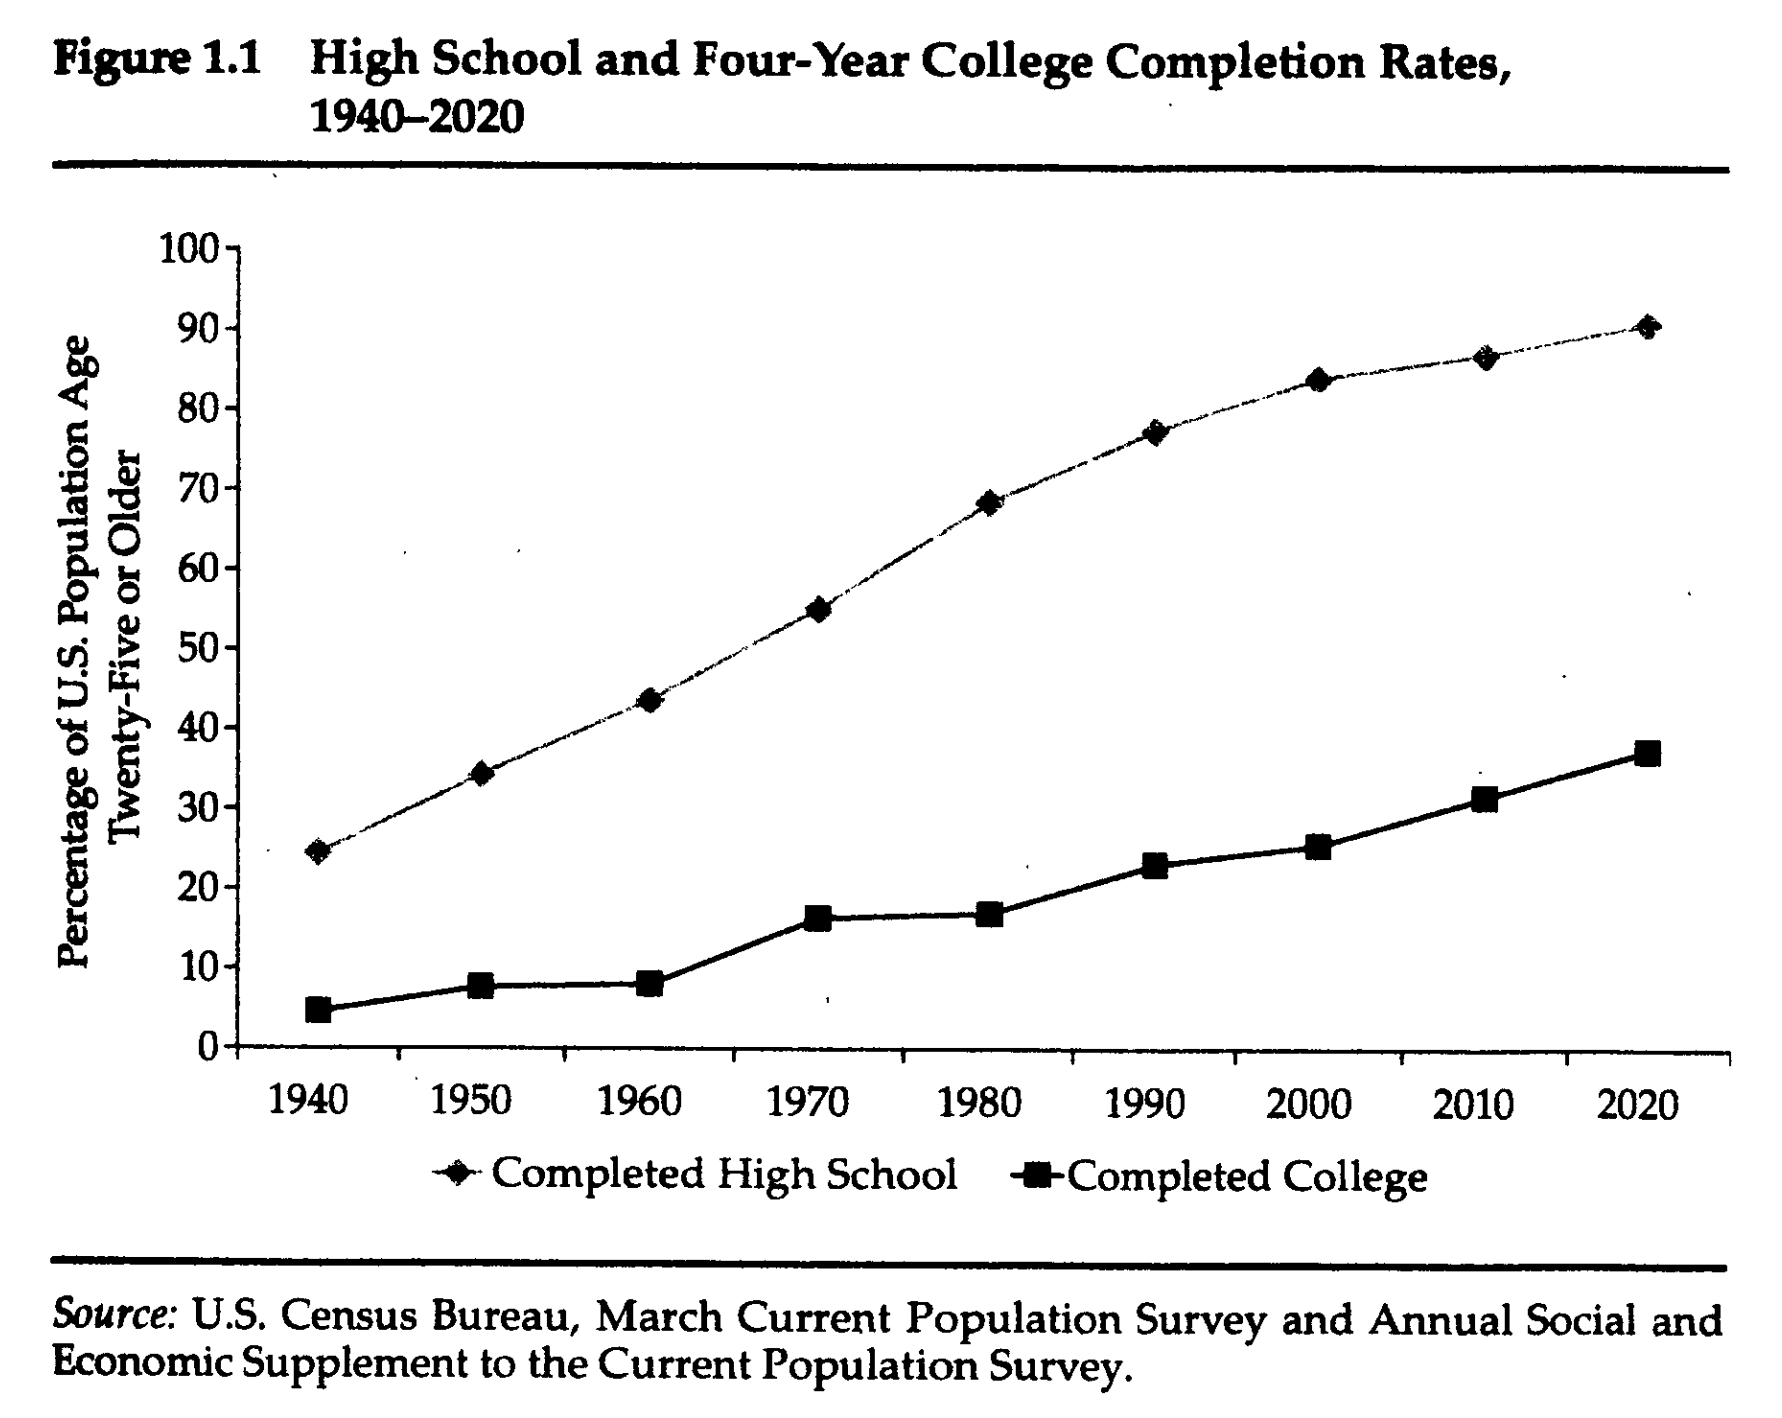
\includegraphics[width = .9\textwidth]{figures/brand_fig1}\\\hfill\mycite{Brand 2023}

\end{frame}

\begin{frame}

We would like to know whether \textbf{college pays off}:\\
does it have positive effects on desired outcomes?

\end{frame}

\begin{frame}{Mathematical notation for two types of claims}


\begin{tikzpicture}[x = \textwidth, y = .8\textheight]
\node at (0,0) {};
\node at (1,1) {};
\node<2->[anchor = north west, align = left] at (.05,1) {People with\\college degrees\\earn more};
\node<2->[anchor = north west, align = left] at (.55,1) {A college degree\\causes\\higher earnings};
\node<3-6>[anchor = north west, align = left] at (0.05,.7) {Two sets of people\\Two treatments};
\only<4->{
\draw[rounded corners, fill = blue, fill opacity = .3] (.05,.3) rectangle (.25,.5) {};
\draw[rounded corners, fill = seagreen, fill opacity = .3] (.25,.1) rectangle (.45,.3) {};
\node[anchor = north, align = center, font = \footnotesize, blue] at (.15, .1) {Outcome\\with college};
\node[anchor = north, align = center, font = \footnotesize, seagreen] at (.35, .1) {Outcome\\without};
\node[anchor = south, rotate = 90, align = center] at (.05, .3) {People};
}
\node<5-7>[anchor = north west, align = left] at (.55,.7) {Same people\\Two treatments};
\only<6->{
\draw[rounded corners, fill = blue, fill opacity = .3] (.55,.1) rectangle (.75,.5) {};
\draw[rounded corners, fill = seagreen, fill opacity = .3] (.75,.1) rectangle (.95,.5) {};
\node[anchor = north, align = center, font = \footnotesize, blue] at (.65, .1) {Outcome\\with college};
\node[anchor = north, align = center, font = \footnotesize, seagreen] at (.85, .1) {Outcome\\without};
\node[anchor = south, rotate = 90, align = center] at (.55, .3) {People};
}
\node<7-> at (.15, .4) {$Y_i$};
\node<7-> at (.35, .2) {$Y_i$};
\node<8-> at (.65, .3) {$Y_i^\text{College}$};
\node<8->[font = \small] at (.85, .3) {$Y_i^\text{Non-college}$};
\only<7->{
\node[anchor = north, align = center] (factual) at (.25,.7) {factual\\outcomes};
\draw[->, thick] (.2,.55) -- (.15,.45);
\draw[->, thick] (.3,.55) -- (.35,.25);
}
\only<8->{
\node[anchor = north, align = center] (potential) at (.75,.7) {potential\\outcomes};
\draw[->, thick] (.7,.55) -- (.65,.35);
\draw[->, thick] (.8,.55) -- (.85,.35);
}
\node<8->[anchor = north east, align = right, font = \footnotesize, gray] at (1,.7) {\href{https://catalog.library.cornell.edu/catalog/12108069}{Imbens \&}\\\href{https://catalog.library.cornell.edu/catalog/12108069}{Rubin}\\\href{https://catalog.library.cornell.edu/catalog/12108069}{2015}};
\end{tikzpicture}

\end{frame}

\begin{frame}{\only<1-3>{The fundamental problem of causal inference}\only<4->{Preview: Solving the problem by assumptions}}
\begin{tikzpicture}[x = \textwidth, y = .8\textheight]
\node at (0,0) {};
\node at (1,1) {};
\node<1-3>[anchor = south east, gray, font = \bf] at (1,0) {\href{https://www.tandfonline.com/doi/abs/10.1080/01621459.1986.10478354}{Holland 1986}};
% Individual outcomes
\node[anchor = north west, font = \bf] at (.05,1) {The data};
\foreach \i in {.5,.7,.8} {
	\draw[fill = blue, opacity = .3, color = blue] (.05,\i) rectangle (.25,\i + .1) {};
}
\foreach \i in {.3,.4,.6} {
	\draw[fill = seagreen, opacity = .3, color = seagreen] (.25,\i) rectangle (.45,\i + .1) {};
}
\node[font = \footnotesize] at (.15,.85) {$Y_\text{Nick}^\text{College}$};
\node[font = \footnotesize] at (.15,.75) {$Y_\text{William}^\text{College}$};
\node[font = \footnotesize] at (.35,.65) {$Y_\text{Rich}^\text{Non-college}$};
\node[font = \footnotesize] at (.15,.55) {$Y_\text{Diego}^\text{College}$};
\node[font = \footnotesize] at (.35,.45) {$Y_\text{Javier}^\text{Non-college}$};
\node[font = \footnotesize] at (.35,.35) {$Y_\text{Jes\'us}^\text{Non-college}$};
\node[anchor = north, align = center, font = \footnotesize, blue] at (.15, .3) {Outcome\\under\\treatment};
\node[anchor = north, align = center, font = \footnotesize, seagreen] at (.35, .3) {Outcome\\under\\control};
\node[anchor = south, rotate = 90, align = center] at (.05, .6) {Each Row is a Person};
% The claim
\onslide<2->{
\node[anchor = north west, font = \bf] at (.55,1) {The claim};
\foreach \i in {.3,.4,.5,.6,.7,.8} {
	\draw[fill = blue, opacity = .3, color = blue] (.55,\i) rectangle (.75,\i + .1) {};
	\draw[fill = seagreen, opacity = .3, color = seagreen] (.75,\i) rectangle (.95,\i + .1) {};
	\draw[<->, thick] (.73,\i + .05) -- (.77,\i + .05);
}
\node[font = \footnotesize] at (.65,.85) {$Y_\text{Nick}^\text{College}$};
\node[font = \footnotesize] at (.85,.85) {$Y_\text{Nick}^\text{Non-college}$};
\node[font = \footnotesize] at (.65,.75) {$Y_\text{William}^\text{College}$};
\node[font = \footnotesize] at (.85,.75) {$Y_\text{William}^\text{Non-college}$};
\node[font = \footnotesize] at (.65,.65) {$Y_\text{Rich}^\text{College}$};
\node[font = \footnotesize] at (.85,.65) {$Y_\text{Rich}^\text{Non-college}$};
\node[font = \footnotesize] at (.65,.55) {$Y_\text{Diego}^\text{College}$};
\node[font = \footnotesize] at (.85,.55) {$Y_\text{Diego}^\text{Non-college}$};
\node[font = \footnotesize] at (.65,.45) {$Y_\text{Javier}^\text{College}$};
\node[font = \footnotesize] at (.85,.45) {$Y_\text{Javier}^\text{Non-college}$};
\node[font = \footnotesize] at (.65,.35) {$Y_\text{Jes\'us}^\text{College}$};
\node[font = \footnotesize] at (.85,.35) {$Y_\text{Jes\'us}^\text{Non-college}$};
\node[anchor = north, align = center, font = \footnotesize, blue] at (.65, .3) {Outcome\\under\\treatment};
\node[anchor = north, align = center, font = \footnotesize, seagreen] at (.85, .3) {Outcome\\under\\control};
}
\node<3>[anchor = north west] at (0,.06) {Counterfactuals are \textbf{not observed}};
\onslide<3->{
\node[font = \footnotesize] at (.35,.85) {?};
\node[font = \footnotesize] at (.35,.75) {?};
\node[font = \footnotesize] at (.15,.65) {?};
\node[font = \footnotesize] at (.35,.55) {?};
\node[font = \footnotesize] at (.15,.45) {?};
\node[font = \footnotesize] at (.15,.35) {?};
}
\draw<5-> (.05,.6) rectangle (.45,.9);
\draw<5-> (.05,.3) rectangle (.45,.6);
\draw<6->[->, thick] (.3, .68) to[out = 90, in = 215] (.33,.73);
\draw<6->[->, thick] (.3, .68) to[out = 90, in = 215] (.33,.83);
\draw<7->[->, thick] (.1, .83) to[out = 215, in = 150] (.13,.65);
\draw<7->[->, thick] (.1, .73) to[out = 215, in = 150] (.13,.65);
\draw<8->[->, thick] (.116, .53) to[out = 270, in = 150] (.14,.47);
\draw<8->[->, thick] (.116, .53) to[out = 270, in = 150] (.14,.37);
\draw<9->[->, thick] (.3, .47) to[out = 115, in = 210] (.33,.53);
\draw<9->[->, thick] (.28, .37) to[out = 145, in = 210] (.33,.53);
\end{tikzpicture}
\end{frame}

\begin{frame}{Quick review} \pause

\begin{enumerate}
\item causal claims involve potential outcomes: $Y^a$
\item not all potential outcomes are observed
\item causal inference is a missing data problem
\end{enumerate} %\vskip .2in
%\textbf{Next:} In what ways should Nick's matches look like him?

\end{frame}

\section{Exchangeability}

\begin{frame}{Exchangeable sampling from a population}
\pause
\begin{tikzpicture}[x = \textwidth, y = .9\textheight]
% POPULATION
\node[anchor = north, font = \bf, color = ucla, align = center] at (.15,1) {Population\\Outcomes};
\foreach \i in {.3,.4,.5,.6,.7,.8} {
	\draw[fill = ucla, draw = white] (.08,\i - .05) rectangle (.22,\i + .05) {};
}
\node[font = {\bf}, white] at (.15,.8) {$Y_\text{Maria}$};
\node[font = {\bf}, white] at (.15,.7) {$Y_\text{William}$};
\node[font = {\bf}, white] at (.15,.6) {$Y_\text{Rich}$};
\node[font = {\bf}, white] at (.15,.5) {$Y_\text{Sarah}$};
\node[font = {\bf}, white] at (.15,.4) {$Y_\text{Alondra}$};
\node[font = {\bf}, white] at (.15,.3) {$Y_\text{Jes\'us}$};
\pause
% RANDOMIZATION
\node[anchor = north, font = \bf, color = ucla, align = center] at (.4,1) {Randomized\\Sampling};
%\foreach \i in {.3,.4,.5,.6,.7,.8} {
%	\draw[fill = ucla, draw = white] (.4,\i) rectangle (6,\i + .1) {};
%}
\node[font = {\bf}, anchor = east, ucla] at (.5,.8) {$S_\text{Maria} = 1$};
\node[font = {\bf}, anchor = east, ucla] at (.5,.7) {$S_\text{William} = 0$};
\node[font = {\bf}, anchor = east, ucla] at (.5,.6) {$S_\text{Rich} = 0$};
\node[font = {\bf}, anchor = east, ucla] at (.5,.5) {$S_\text{Sarah} = 1$};
\node[font = {\bf}, anchor = east, ucla] at (.5,.4) {$S_\text{Alondra} = 0$};
\node[font = {\bf}, anchor = east, ucla] at (.5,.3) {$S_\text{Jes\'us} = 1$};
\pause
% SAMPLE
\node[anchor = north, font = \bf, color = ucla, align = center] at (.62,1) {Sampled\\Outcomes};
\foreach \i in {.3,.5,.8} {
	\draw[fill = ucla, draw = white] (.55,\i - .05) rectangle (.69,\i + .05) {};
}
\node[font = {\bf}, white] at (.62,.8) {$Y_\text{Maria}$};
%\node[font = {\bf}, white] at (.75,.75) {$Y_\text{William}$};
%\node[font = {\bf}, white] at (.75,.65) {$Y_\text{Rich}$};
\node[font = {\bf}, white] at (.62,.5) {$Y_\text{Sarah}$};
%\node[font = {\bf}, white] at (.75,.45) {$Y_\text{Alondra}$};
\node[font = {\bf}, white] at (.62,.3) {$Y_\text{Jes\'us}$};
%\draw[fill = darkgray] (.75,0) rectangle (2,1);
\pause
\node[anchor = north west, align = left] at (.75,1) {\textbf{Estimator:}\\Estimate the\\population mean\\by the sample mean};
\node[anchor = north west, align = left] at (.75,.65) {\textbf{Key assumption}:\\Sampled and\\unsampled units\\are \textbf{exchangeable}\\due to random\\sampling};
\node[anchor = north west, align = left] at (.75,.27) {$Y\indep S$};
\end{tikzpicture}
\end{frame}

\begin{frame}
Now suppose our population all participate\\in a randomized experiment with\\treatment ($A = 1$) and control ($A = 0$) conditions
\end{frame}


\begin{frame}{Exchangeable treatment assignment} %Y1

\begin{tikzpicture}[x = \textwidth, y = .9\textheight]
% POPULATION
\node[anchor = north, font = \bf, color = ucla, align = center] at (.15,1.05) {Population\\Potential\\Outcomes};
\foreach \i in {.3,.4,.5,.6,.7,.8} {
	\draw[fill = ucla, draw = white] (.08,\i - .05) rectangle (.22,\i + .05) {};
}
\node[font = {\bf}, white] at (.15,.8) {$Y^1_\text{Maria}$};
\node[font = {\bf}, white] at (.15,.7) {$Y^1_\text{William}$};
\node[font = {\bf}, white] at (.15,.6) {$Y^1_\text{Rich}$};
\node[font = {\bf}, white] at (.15,.5) {$Y^1_\text{Sarah}$};
\node[font = {\bf}, white] at (.15,.4) {$Y^1_\text{Alondra}$};
\node[font = {\bf}, white] at (.15,.3) {$Y^1_\text{Jes\'us}$};
\pause
% RANDOMIZATION
\node[anchor = north, font = \bf, color = ucla, align = center] at (.4,1) {Randomized\\Treatment};
%\foreach \i in {.3,.4,.5,.6,.7,.8} {
%	\draw[fill = ucla, draw = white] (.4,\i) rectangle (6,\i + .1) {};
%}
\node[font = {\bf}, anchor = east, ucla] at (.5,.8) {$A_\text{Maria} = 1$};
\node[font = {\bf}, anchor = east, ucla] at (.5,.7) {$A_\text{William} = 0$};
\node[font = {\bf}, anchor = east, ucla] at (.5,.6) {$A_\text{Rich} = 0$};
\node[font = {\bf}, anchor = east, ucla] at (.5,.5) {$A_\text{Sarah} = 1$};
\node[font = {\bf}, anchor = east, ucla] at (.5,.4) {$A_\text{Alondra} = 0$};
\node[font = {\bf}, anchor = east, ucla] at (.5,.3) {$A_\text{Jes\'us} = 1$};
\pause
% SAMPLE
\node[anchor = north, font = \bf, color = ucla, align = center] at (.62,1) {Observed\\Outcomes};
\foreach \i in {.3,.5,.8} {
	\draw[fill = ucla, draw = white] (.55,\i - .05) rectangle (.69,\i + .05) {};
}
\node[font = {\bf}, white] at (.62,.8) {$Y^1_\text{Maria}$};
%\node[font = {\bf}, white] at (.75,.75) {$Y_\text{William}$};
%\node[font = {\bf}, white] at (.75,.65) {$Y_\text{Rich}$};
\node[font = {\bf}, white] at (.62,.5) {$Y^1_\text{Sarah}$};
%\node[font = {\bf}, white] at (.75,.45) {$Y_\text{Alondra}$};
\node[font = {\bf}, white] at (.62,.3) {$Y^1_\text{Jes\'us}$};
%\draw[fill = darkgray] (.75,0) rectangle (2,1);
\pause
\node[anchor = north west, align = left] at (.75,1) {\textbf{Estimator:}\\Estimate the\\population mean\\$\E(Y^1)$ by the\\untreated sample mean};
\node[anchor = north west, align = left] at (.75,.65) {\textbf{Key assumption}:\\Treated and\\untreated units\\are \textbf{exchangeable}\\due to random\\treatment assignment};
\node[anchor = north west, align = left] at (.75,.27) {$Y^1\indep A$};
\end{tikzpicture}
\end{frame}


\begin{frame}{Exchangeable treatment assignment} %Y0

\begin{tikzpicture}[x = \textwidth, y = .9\textheight]
% POPULATION
\node[anchor = north, font = \bf, color = ucla, align = center] at (.15,1.05) {Population\\Potential\\Outcomes};
\foreach \i in {.3,.4,.5,.6,.7,.8} {
	\draw[fill = gold, draw = white] (.08,\i - .05) rectangle (.22,\i + .05) {};
}
\node[font = {\bf}, darkestblue] at (.15,.8) {$Y^0_\text{Maria}$};
\node[font = {\bf}, darkestblue] at (.15,.7) {$Y^0_\text{William}$};
\node[font = {\bf}, darkestblue] at (.15,.6) {$Y^0_\text{Rich}$};
\node[font = {\bf}, darkestblue] at (.15,.5) {$Y^0_\text{Sarah}$};
\node[font = {\bf}, darkestblue] at (.15,.4) {$Y^0_\text{Alondra}$};
\node[font = {\bf}, darkestblue] at (.15,.3) {$Y^0_\text{Jes\'us}$};
% RANDOMIZATION
\node[anchor = north, font = \bf, color = ucla, align = center] at (.4,1) {Randomized\\Treatment};
%\foreach \i in {.3,.4,.5,.6,.7,.8} {
%	\draw[fill = ucla, draw = white] (.4,\i) rectangle (6,\i + .1) {};
%}
\node[font = {\bf}, anchor = east, ucla] at (.5,.8) {$A_\text{Maria} = 1$};
\node[font = {\bf}, anchor = east, ucla] at (.5,.7) {$A_\text{William} = 0$};
\node[font = {\bf}, anchor = east, ucla] at (.5,.6) {$A_\text{Rich} = 0$};
\node[font = {\bf}, anchor = east, ucla] at (.5,.5) {$A_\text{Sarah} = 1$};
\node[font = {\bf}, anchor = east, ucla] at (.5,.4) {$A_\text{Alondra} = 0$};
\node[font = {\bf}, anchor = east, ucla] at (.5,.3) {$A_\text{Jes\'us} = 1$};
% SAMPLE
\node[anchor = north, font = \bf, color = ucla, align = center] at (.62,1) {Observed\\Outcomes};
\foreach \i in {.4,.6,.7} {
	\draw[fill = gold, draw = white] (.55,\i - .05) rectangle (.69,\i + .05) {};
}
%\node[font = {\bf}, white] at (.62,.8) {$Y^1_\text{Maria}$};
\node[font = {\bf}, darkestblue] at (.62,.7) {$Y^0_\text{William}$};
\node[font = {\bf}, darkestblue] at (.62,.6) {$Y^0_\text{Rich}$};
%\node[font = {\bf}, white] at (.62,.5) {$Y^1_\text{Sarah}$};
\node[font = {\bf}, darkestblue] at (.62,.4) {$Y^0_\text{Alondra}$};
%\node[font = {\bf}, white] at (.62,.3) {$Y^1_\text{Jes\'us}$};
\node[anchor = north west, align = left] at (.75,1) {\textbf{Estimator:}\\Estimate the\\population mean\\$\E(Y^0)$ by the\\untreated sample mean};
\node[anchor = north west, align = left] at (.75,.65) {\textbf{Key assumption}:\\Treated and\\untreated units\\are \textbf{exchangeable}\\due to random\\treatment assignment};
\node[anchor = north west, align = left] at (.75,.27) {$Y^0\indep A$};
\end{tikzpicture}
\end{frame}

\begin{frame}{Exchangeable treatment assignment} %Y0 AND Y1

\begin{tikzpicture}[x = \textwidth, y = .9\textheight]
% POPULATION
\node[anchor = north, font = \bf, color = ucla, align = center] at (.23,1.05) {Population\\Potential\\Outcomes};
\foreach \i in {.3,.4,.5,.6,.7,.8} {
	\draw[fill = ucla, draw = white] (.08,\i - .05) rectangle (.22,\i + .05) {};
	\draw[fill = gold, draw = white] (.24,\i - .05) rectangle (.38,\i + .05) {};
}
\node[font = {\bf}, white] at (.15,.8) {$Y^1_\text{Maria}$};
\node[font = {\bf}, white] at (.15,.7) {$Y^1_\text{William}$};
\node[font = {\bf}, white] at (.15,.6) {$Y^1_\text{Rich}$};
\node[font = {\bf}, white] at (.15,.5) {$Y^1_\text{Sarah}$};
\node[font = {\bf}, white] at (.15,.4) {$Y^1_\text{Alondra}$};
\node[font = {\bf}, white] at (.15,.3) {$Y^1_\text{Jes\'us}$};
\node[font = {\bf}, darkestblue] at (.31,.8) {$Y^0_\text{Maria}$};
\node[font = {\bf}, darkestblue] at (.31,.7) {$Y^0_\text{William}$};
\node[font = {\bf}, darkestblue] at (.31,.6) {$Y^0_\text{Rich}$};
\node[font = {\bf}, darkestblue] at (.31,.5) {$Y^0_\text{Sarah}$};
\node[font = {\bf}, darkestblue] at (.31,.4) {$Y^0_\text{Alondra}$};
\node[font = {\bf}, darkestblue] at (.31,.3) {$Y^0_\text{Jes\'us}$};
% RANDOMIZATION
\node[anchor = north, font = \bf, color = ucla, align = center] at (.51,1) {Randomized\\Treatment};
%\foreach \i in {.3,.4,.5,.6,.7,.8} {
%	\draw[fill = ucla, draw = white] (.4,\i) rectangle (6,\i + .1) {};
%}
\node[font = {\bf}, anchor = east, ucla] at (.61,.8) {$A_\text{Maria} = 1$};
\node[font = {\bf}, anchor = east, ucla] at (.61,.7) {$A_\text{William} = 0$};
\node[font = {\bf}, anchor = east, ucla] at (.61,.6) {$A_\text{Rich} = 0$};
\node[font = {\bf}, anchor = east, ucla] at (.61,.5) {$A_\text{Sarah} = 1$};
\node[font = {\bf}, anchor = east, ucla] at (.61,.4) {$A_\text{Alondra} = 0$};
\node[font = {\bf}, anchor = east, ucla] at (.61,.3) {$A_\text{Jes\'us} = 1$};
% SAMPLE
\node[anchor = north, font = \bf, color = ucla, align = center] at (.83,1) {Observed\\Outcomes};
\foreach \i in {.3,.5,.8} {
	\draw[fill = ucla, draw = white] (.68,\i - .05) rectangle (.82,\i + .05) {};
}
\foreach \i in {.4,.6,.7} {
	\draw[fill = gold, draw = white] (.84,\i - .05) rectangle (.98,\i + .05) {};
}
\node[font = {\bf}, white] at (.75,.8) {$Y^1_\text{Maria}$};
\node[font = {\bf}, darkestblue] at (.91,.7) {$Y^0_\text{William}$};
\node[font = {\bf}, darkestblue] at (.91,.6) {$Y^0_\text{Rich}$};
\node[font = {\bf}, white] at (.75,.5) {$Y^1_\text{Sarah}$};
\node[font = {\bf}, darkestblue] at (.91,.4) {$Y^0_\text{Alondra}$};
\node[font = {\bf}, white] at (.75,.3) {$Y^1_\text{Jes\'us}$};
%\node[anchor = north west, align = left] at (.75,1) {\textbf{Estimator:}\\Estimate the\\population mean\\$\E(Y^0)$ by the\\untreated sample mean};
%\node[anchor = north west, align = left] at (.75,.65) {\textbf{Key assumption}:\\Treated and\\untreated units\\are \textbf{exchangeable}\\due to random\\treatment assignment};
%\node[anchor = north west, align = left] at (.75,.27) {$Y^0\indep A$};
\end{tikzpicture}
\end{frame}

\begin{frame}{Exchangeable treatment assignment}
\textbf{Causal Estimand:}\\(expected outcome if assigned to treatment) \\
${}-{}$ (expected outcome if assigned to control)
$$
\E\left(Y^1\right) - \E\left(Y^0\right)
$$ \vskip .1in
\textbf{Exchangeability Assumption}:\\
Potential outcomes are independent of treatment assignment \\
$$\{Y^0,Y^1\}\indep A$$ \vskip .1in
\textbf{Empirical Estimand:}\\
(expected outcome among the treated)\\
$-$ (expected outcome among the untreated)
$$\E(Y\mid A = 1) - \E(Y\mid A = 0)$$
\end{frame}

\begin{frame}{Exchangeable treatment assignment: Proof}
$$\begin{aligned}
&\E\left(Y^1\right) - \E\left(Y^0\right) \\
&= \E\left(Y^1\mid A = 1\right) - \E\left(Y^0\mid A = 0\right) &\onslide<3->{\text{by exchangeability}}\\
&= \E\left(Y\mid A = 1\right) - \E\left(Y\mid A = 0\right) &\onslide<2->{\text{by consistency}}
\end{aligned}$$ \vskip .2in \pause \pause \pause
This is an example of \textbf{causal identification}: \\
using assumptions to arrive at an empirical quantity\\(involving only factual random variables, no potential outcomes)\\that equals our causal estimand if the assumptions hold \vskip .2in
The causal estimand $\E(Y^1) - \E(Y^0)$ is \textbf{identified} by the empirical estimand $\E(Y\mid A = 1) - \E(Y\mid A = 0)$
\end{frame}

\begin{frame}{Potential outcome exercise: Covid vaccines} \pause
% from Sam
Suppose we know the following pieces of information:
{\small
\begin{itemize}
\item Martha was vaccinated against Covid.\\Martha tested negative 6 months later.
\item Ezra was not vaccinated against Covid.\\Ezra tested positive 6 months later.
\end{itemize} \pause
Which cells have known values? What are the values?
}

\begin{table}
  \renewcommand*{\arraystretch}{2}
\begin{tabular}[t]{c|c|c| c|c}
  & $A_i$ & $Y_i$ & $Y_i^{\text{Vaccinated}}$ & $Y_i^{\text{Unvaccinated}}$\\
\hline
Martha & \qquad \qquad \qquad & \qquad \qquad \qquad & \qquad & \qquad\\ \hline
Ezra & \qquad \qquad & \qquad \qquad & \qquad & \qquad\\
\end{tabular}
\end{table}

\end{frame}

\begin{frame}{Experiments vs observational studies}
Suppose we gathered data by surveying individuals in Fall of 2021
    \begin{itemize}
        \item Vaccinated for covid ($A_i = 1$) or not ($A_i = 0$)
        \item Tested positive for Covid in 2021: yes ($Y_i = 1$) or no ($Y_i=0$)
     \end{itemize}
\end{frame}

\begin{frame}{Experiments vs observational studies}
We observe evidence
     \begin{itemize}
         \item Of the individuals who are \textbf{vaccinated} ($A_i = 1$),\\50\% had a positive Covid test ($Y_i = 1$)
         \item Of the individuals who are \textbf{not vaccinated} ($A_i = 0$),\\70\% had a positive Covid test ($Y_i = 1$) 
\end{itemize} \pause
How might a vaccine skeptic explain the data? 
\end{frame}

\begin{frame}{Experiments vs observational studies}
Experiment designed by Pfizer \textbf{randomly assign} each individual (43,000 total) into two groups\footnote{Polack et. al. NEJM 2020}:
\begin{itemize}
        \item Two doses of BNT162b2 vaccine 21 days apart
        \item Two doses of placebo 21 days apart
        \item Whether a positive Covid test was recorded between 7 days and 14 weeks after the injection
\end{itemize}
\vspace{1em}

\pause
     \begin{itemize}
         \item Of the individuals who were given the vaccine ($A_i = 1$), 0.04\% had a positive Covid test ($Y_i = 1$)
         \item Of the individuals who were given the placebo ($A_i = 0$), 0.9\% had a positive Covid test ($Y_i = 1$)
         \item Individuals who received the placebo were $\approx 20$ times more likely to get Covid 
     \end{itemize}

\pause \vspace{1em}
\textbf{Do the skeptic's objections still hold?}

\end{frame}

\begin{frame}{Why experiments ``work'': Exchangeability}

\begin{figure}
    \centering
    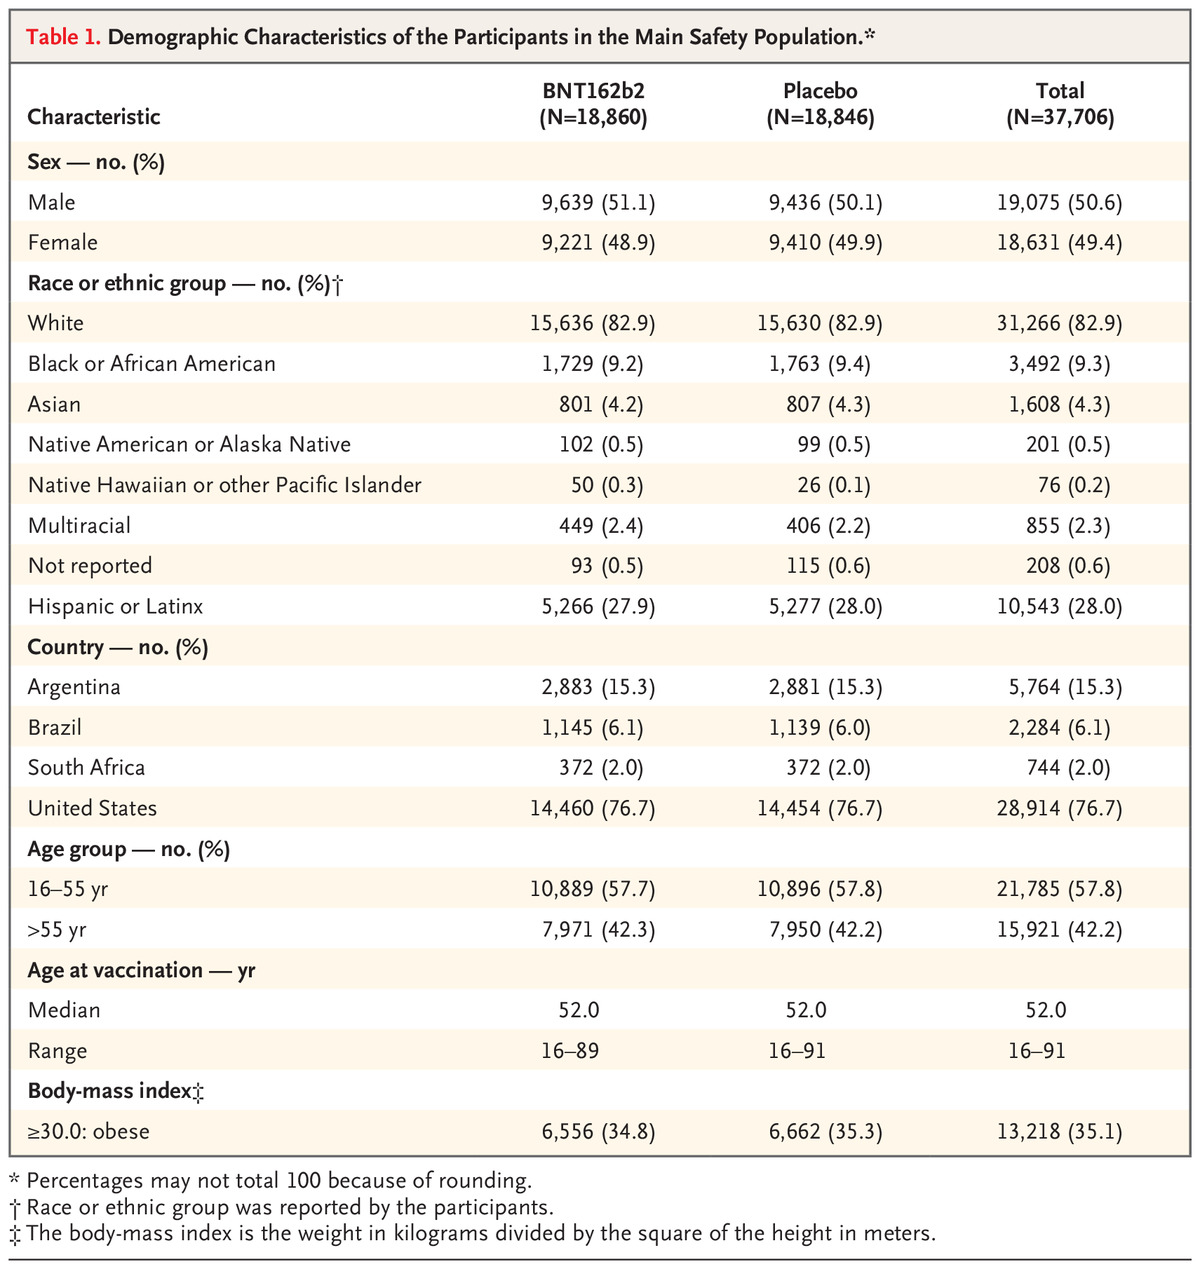
\includegraphics[scale = .18]{figures/pfizer_balance.jpg}
\end{figure}

\end{frame}

\begin{frame}{Why experiments ``work'': Exchangeability}

In random experiments, the distribution of \textbf{potential outcomes} for those who are treated and those who are not treated (control group) are identically distributed!

$$\{Y^1,Y^0\}\indep A$$

\vspace{2em}
This is \textbf{exchangeability} \vskip .2in

\textbf{Question.} Does exchangeability imply $Y\indep A$?

\end{frame}

\begin{frame}{Why experiments ``work'': Exchangeability}

Exchangeability is about \textbf{potential} rather than \textbf{observed} outcomes
$$\{Y^0,Y^1\}\indep A\qquad\text{rather than}\qquad Y\not\indep A$$
 \pause
\begin{itemize}
\item Potential outcomes are independent of treatment $\{Y^0,Y^1\}\indep A$
\begin{itemize}
\item Example: Risk of covid under no vaccine ($Y^0$) is the same for those with and without a vaccine
\end{itemize} \pause
\item Observed outcomes are not independent of treatment $Y\not\indep A$
\begin{itemize}
\item Example: Risk of covid is lower for those with the vaccine
\item Why? Because for them $Y = Y^1$. For others, $Y = Y^0$.
\item If $A$ affects $Y$, then $Y\not\indep A$
\end{itemize}
\end{itemize} \pause
Under exchangeability, the only reason $Y\not\indep A$ is if $A$ causes $Y$.
\end{frame}

\begin{frame}
\huge
Review of exchangeability
\end{frame}

\begin{frame}{Exchangeable sampling from a population}
\begin{tikzpicture}[x = \textwidth, y = .9\textheight]
% POPULATION
\node[anchor = north, font = \bf, color = ucla, align = center] at (.15,1) {Population\\Outcomes};
\foreach \i in {.3,.4,.5,.6,.7,.8} {
	\draw[fill = ucla, draw = white] (.08,\i - .05) rectangle (.22,\i + .05) {};
}
\node[font = {\bf}, white] at (.15,.8) {$Y_\text{Maria}$};
\node[font = {\bf}, white] at (.15,.7) {$Y_\text{William}$};
\node[font = {\bf}, white] at (.15,.6) {$Y_\text{Rich}$};
\node[font = {\bf}, white] at (.15,.5) {$Y_\text{Sarah}$};
\node[font = {\bf}, white] at (.15,.4) {$Y_\text{Alondra}$};
\node[font = {\bf}, white] at (.15,.3) {$Y_\text{Jes\'us}$};
% RANDOMIZATION
\node[anchor = north, font = \bf, color = ucla, align = center] at (.4,1) {Randomized\\Sampling};
%\foreach \i in {.3,.4,.5,.6,.7,.8} {
%	\draw[fill = ucla, draw = white] (.4,\i) rectangle (6,\i + .1) {};
%}
\node[font = {\bf}, anchor = east, ucla] at (.5,.8) {$S_\text{Maria} = 1$};
\node[font = {\bf}, anchor = east, ucla] at (.5,.7) {$S_\text{William} = 0$};
\node[font = {\bf}, anchor = east, ucla] at (.5,.6) {$S_\text{Rich} = 0$};
\node[font = {\bf}, anchor = east, ucla] at (.5,.5) {$S_\text{Sarah} = 1$};
\node[font = {\bf}, anchor = east, ucla] at (.5,.4) {$S_\text{Alondra} = 0$};
\node[font = {\bf}, anchor = east, ucla] at (.5,.3) {$S_\text{Jes\'us} = 1$};
% SAMPLE
\node[anchor = north, font = \bf, color = ucla, align = center] at (.62,1) {Sampled\\Outcomes};
\foreach \i in {.3,.5,.8} {
	\draw[fill = ucla, draw = white] (.55,\i - .05) rectangle (.69,\i + .05) {};
}
\node[font = {\bf}, white] at (.62,.8) {$Y_\text{Maria}$};
%\node[font = {\bf}, white] at (.75,.75) {$Y_\text{William}$};
%\node[font = {\bf}, white] at (.75,.65) {$Y_\text{Rich}$};
\node[font = {\bf}, white] at (.62,.5) {$Y_\text{Sarah}$};
%\node[font = {\bf}, white] at (.75,.45) {$Y_\text{Alondra}$};
\node[font = {\bf}, white] at (.62,.3) {$Y_\text{Jes\'us}$};
%\draw[fill = darkgray] (.75,0) rectangle (2,1);
\node[anchor = north west, align = left] at (.75,1) {\textbf{Estimator:}\\Estimate the\\population mean\\by the sample mean};
\node[anchor = north west, align = left] at (.75,.65) {\textbf{Key assumption}:\\Sampled and\\unsampled units\\are \textbf{exchangeable}\\due to random\\sampling};
\node[anchor = north west, align = left] at (.75,.27) {$Y\indep S$};
\end{tikzpicture}
\end{frame}

\begin{frame}{Exchangeable treatment assignment} %Y0 AND Y1

\begin{tikzpicture}[x = \textwidth, y = .9\textheight]
% POPULATION
\node[anchor = north, font = \bf, color = ucla, align = center] at (.23,1.05) {Population\\Potential\\Outcomes};
\foreach \i in {.3,.4,.5,.6,.7,.8} {
	\draw[fill = ucla, draw = white] (.08,\i - .05) rectangle (.22,\i + .05) {};
	\draw[fill = gold, draw = white] (.24,\i - .05) rectangle (.38,\i + .05) {};
}
\node[font = {\bf}, white] at (.15,.8) {$Y^1_\text{Maria}$};
\node[font = {\bf}, white] at (.15,.7) {$Y^1_\text{William}$};
\node[font = {\bf}, white] at (.15,.6) {$Y^1_\text{Rich}$};
\node[font = {\bf}, white] at (.15,.5) {$Y^1_\text{Sarah}$};
\node[font = {\bf}, white] at (.15,.4) {$Y^1_\text{Alondra}$};
\node[font = {\bf}, white] at (.15,.3) {$Y^1_\text{Jes\'us}$};
\node[font = {\bf}, darkestblue] at (.31,.8) {$Y^0_\text{Maria}$};
\node[font = {\bf}, darkestblue] at (.31,.7) {$Y^0_\text{William}$};
\node[font = {\bf}, darkestblue] at (.31,.6) {$Y^0_\text{Rich}$};
\node[font = {\bf}, darkestblue] at (.31,.5) {$Y^0_\text{Sarah}$};
\node[font = {\bf}, darkestblue] at (.31,.4) {$Y^0_\text{Alondra}$};
\node[font = {\bf}, darkestblue] at (.31,.3) {$Y^0_\text{Jes\'us}$};
% RANDOMIZATION
\node[anchor = north, font = \bf, color = ucla, align = center] at (.51,1) {Randomized\\Treatment};
%\foreach \i in {.3,.4,.5,.6,.7,.8} {
%	\draw[fill = ucla, draw = white] (.4,\i) rectangle (6,\i + .1) {};
%}
\node[font = {\bf}, anchor = east, ucla] at (.61,.8) {$A_\text{Maria} = 1$};
\node[font = {\bf}, anchor = east, ucla] at (.61,.7) {$A_\text{William} = 0$};
\node[font = {\bf}, anchor = east, ucla] at (.61,.6) {$A_\text{Rich} = 0$};
\node[font = {\bf}, anchor = east, ucla] at (.61,.5) {$A_\text{Sarah} = 1$};
\node[font = {\bf}, anchor = east, ucla] at (.61,.4) {$A_\text{Alondra} = 0$};
\node[font = {\bf}, anchor = east, ucla] at (.61,.3) {$A_\text{Jes\'us} = 1$};
% SAMPLE
\node[anchor = north, font = \bf, color = ucla, align = center] at (.83,1) {Observed\\Outcomes};
\foreach \i in {.3,.5,.8} {
	\draw[fill = ucla, draw = white] (.68,\i - .05) rectangle (.82,\i + .05) {};
}
\foreach \i in {.4,.6,.7} {
	\draw[fill = gold, draw = white] (.84,\i - .05) rectangle (.98,\i + .05) {};
}
\node[font = {\bf}, white] at (.75,.8) {$Y^1_\text{Maria}$};
\node[font = {\bf}, darkestblue] at (.91,.7) {$Y^0_\text{William}$};
\node[font = {\bf}, darkestblue] at (.91,.6) {$Y^0_\text{Rich}$};
\node[font = {\bf}, white] at (.75,.5) {$Y^1_\text{Sarah}$};
\node[font = {\bf}, darkestblue] at (.91,.4) {$Y^0_\text{Alondra}$};
\node[font = {\bf}, white] at (.75,.3) {$Y^1_\text{Jes\'us}$};
%\node[anchor = north west, align = left] at (.75,1) {\textbf{Estimator:}\\Estimate the\\population mean\\$\E(Y^0)$ by the\\untreated sample mean};
%\node[anchor = north west, align = left] at (.75,.65) {\textbf{Key assumption}:\\Treated and\\untreated units\\are \textbf{exchangeable}\\due to random\\treatment assignment};
%\node[anchor = north west, align = left] at (.75,.27) {$Y^0\indep A$};
\end{tikzpicture}
\end{frame}

\section{Conditional Exchangeability}

\begin{frame}
\huge A \textbf{conditionally} randomized experiment
\end{frame}

\begin{frame}
\onslide<2->{\Large Does exchangeability hold? How would you analyze?\vskip .1in}
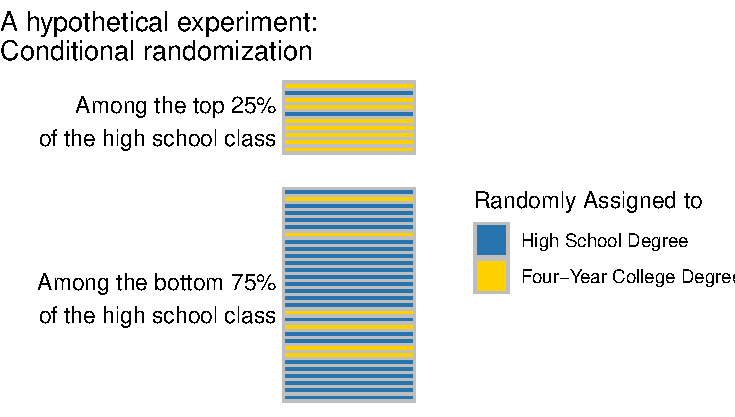
\includegraphics[width = \textwidth]{figures/conditional_randomization} \\
Outcome: Employed at age 40

\end{frame}

\begin{frame}{Conditional randomization: Exchangeability does not hold}

\begin{tikzpicture}[x = \textwidth, y =.8\textheight]
\node at (0,0) {};
\node at (1,1) {};
\node[anchor = south] at (.5,0) {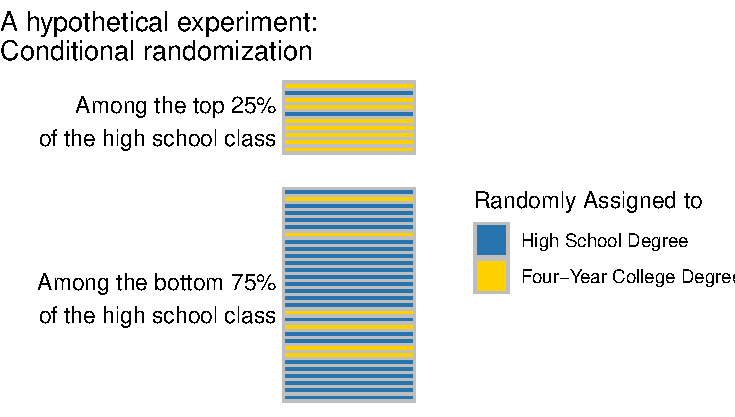
\includegraphics[width = .5\textwidth]{figures/conditional_randomization}};
\node<2->[anchor = north west, align = left, text width = \textwidth] at (0,1) {Treated units are more likely to have done well in high school};
\node<3->[anchor = north west, align = left, text width = \textwidth] at (0,.9) {Those who do well in high school are more likely to be employed at age 40 even without college};
\node<4->[anchor = north, font = \Large] at (.5,.75) {$\{Y^1,Y^0\}\not\indep A$};
\end{tikzpicture}

\end{frame}

\begin{frame}{Conditional randomization: Analyze within subgroups}

\begin{tikzpicture}[x = \textwidth, y =.8\textheight]
\node at (0,0) {};
\node at (1,1) {};
\node[anchor = south] at (.5,0) {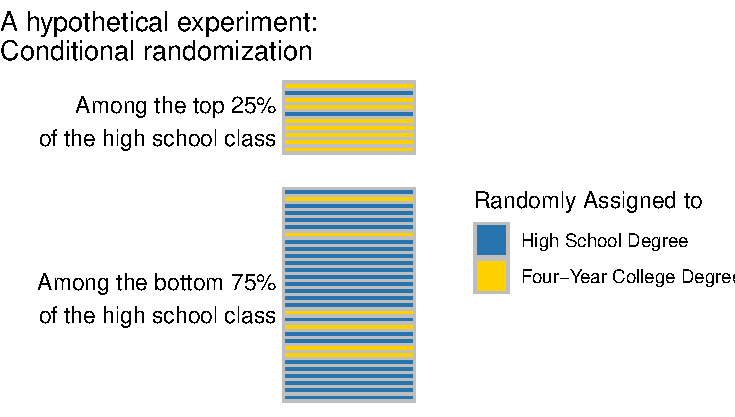
\includegraphics[width = .5\textwidth]{figures/conditional_randomization}};
\node<2->[anchor = north west, align = left, text width = \textwidth] at (0,1) {Among top 25\%, simple random experiment.\\Among bottom 75\%, simple random experiment.};
\node<3->[anchor = north west, align = left, text width = \textwidth] at (0,.85) {Conditional exchangeability:};
\node<3->[anchor = north, font = \Large] at (.5,.75) {$\underbrace{\{Y^1,Y^0\}}_{\substack{\text{Potential}\\\text{Outcomes}}} \underbrace{\indep}_{\substack{\text{Are}\\\text{Independent of}}} \underbrace{A}_\text{Treatment} \underbrace{\mid}_{\substack{\text{Within}\\\text{Subgroups}}} \underbrace{X}_\text{of X}$};
\end{tikzpicture}

\end{frame}

\begin{frame}{Conditional average treatment effects}

We get two estimates. Average effect of college on employment
\begin{itemize}
\item among those in the top 25\% of their high school class
\item among those in the bottom 75\% of their high school class
\end{itemize} \vskip .2in
These are \textbf{conditional average treatment effects}
$$
\underbrace{\tau(x)}_{\substack{\text{Conditional}\\\text{Average}\\\text{Treatment}\\\text{Effect}\\\text{(CATE)}}} = \underbrace{\text{E}}_{\substack{\text{Expected}\\\text{value of}}}\bigg(\underbrace{Y^1-Y^0}_\text{treatment effect} \quad \underbrace{\mid}_{\substack{\text{within the}\\\text{subgroup}\\\text{for whom}}} \quad \underbrace{\vec{X} = \vec{x}}_{\substack{\text{the predictors }\vec{X}\\\text{take the value }\vec{x}}}\bigg)
$$

\end{frame}

\begin{frame}{Effect heterogeneity: CATEs differ across subgroups}

Why might the effect of college on future employment
\begin{itemize}
\item be larger for those from the top 25\% of the high school class?
\item be larger for those from the bottom 75\% of the high school class?
\end{itemize}

\end{frame}

\begin{frame}{Effect heterogeneity and policy}

Suppose we study (college $\rightarrow$ employment) in two subgroups
\begin{itemize}
\item Advantaged subgroup
\begin{itemize}
\item Both parents finished college
\item Top quartile of family income at age 14
\item Took college prep courses
\end{itemize}
\item Disadvantaged subgroup
\begin{itemize}
\item Neither parent finished college
\item Bottom quartile of family income at age 14
\item Took college prep courses
\end{itemize}
\end{itemize} \vskip .1in
Discuss:
\begin{enumerate}
\item Whose CATE would be larger?
\item How might the difference inform policy?
\end{enumerate}

\end{frame}

\begin{frame}
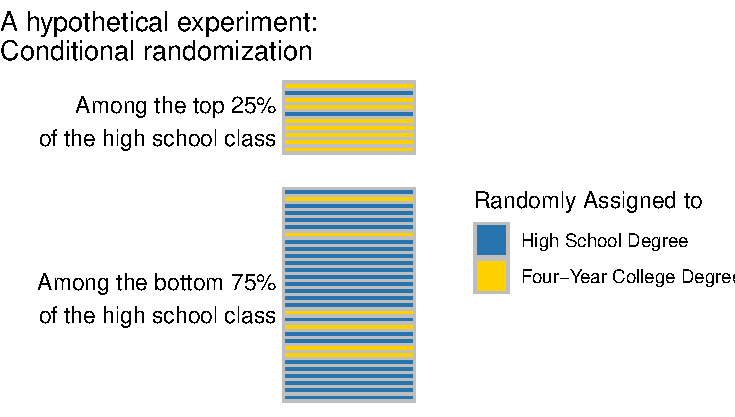
\includegraphics[width = \textwidth]{figures/conditional_randomization} \\
Outcome: Employed at age 40

\end{frame}

\section{DAGs}

\subsection{Nodes and Edges}

\begin{frame}[t]{Elements of a Directed Acyclic Graph (DAG)}

\begin{center}
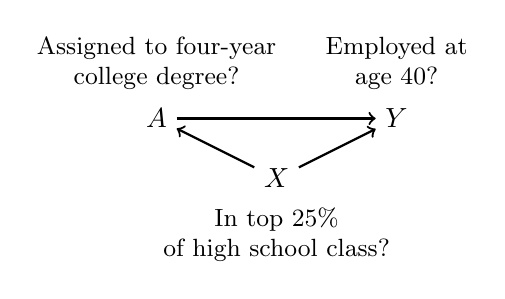
\begin{tikzpicture}[x = .3in, y = .3in]
    \node at (-3,0) {};
    \node at (3,0) {};
    \node (x) at (0,-1) {$X$};
    \node (a) at (-2,0) {$A$};
    \node (y) at (2,0) {$Y$};
    \draw[->, thick] (x) -- (a);
    \draw[->, thick] (a) -- (y);
    \draw[->, thick] (x) -- (y);
        % Labels
    \node[anchor = north, font = \small, align = center] at (x.south) {In top 25\%\\of high school class?};
    \node[anchor = south, font = \small, align = center] at (a.north) {Assigned to four-year\\college degree?};
    \node[anchor = south, font = \small, align = center] at (y.north) {Employed at\\age 40?};
  \end{tikzpicture}
\end{center}
  
  \begin{itemize}
  \item \textbf{Nodes} ($X,A,Y$) are random variables
  \item \textbf{Edges} ($\rightarrow$) are causal relationships.
  \begin{itemize}
  \item $X$ has a causal effect on $A$
  \item $X$ has a causal effect on $Y$
  \item $A$ has a causal effect on $Y$
  \end{itemize}
  \end{itemize}
  
\end{frame}

\begin{frame}[t]{Elements of a Directed Acyclic Graph (DAG)}

\begin{center}
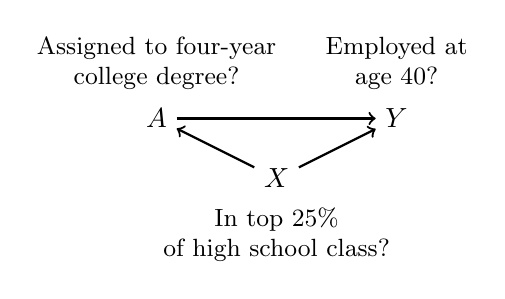
\begin{tikzpicture}[x = .3in, y = .3in]
    \node at (-3,0) {};
    \node at (3,0) {};
    \node (x) at (0,-1) {$X$};
    \node (a) at (-2,0) {$A$};
    \node (y) at (2,0) {$Y$};
    \draw[->, thick] (x) -- (a);
    \draw[->, thick] (a) -- (y);
    \draw[->, thick] (x) -- (y);
        % Labels
    \node[anchor = north, font = \small, align = center] at (x.south) {In top 25\%\\of high school class?};
    \node[anchor = south, font = \small, align = center] at (a.north) {Assigned to four-year\\college degree?};
    \node[anchor = south, font = \small, align = center] at (y.north) {Employed at\\age 40?};
  \end{tikzpicture}
\end{center}

A \textbf{path} is a sequence of edges connecting two nodes. \vskip .1in \pause
Between $A$ and $Y$, what are the two paths? \pause
\begin{itemize}
\item $A\rightarrow Y$
\item $A\leftarrow X \rightarrow Y$
\end{itemize}

\end{frame}

\subsection{Causal Paths}

\begin{frame}{Causal path: A path with arrows pointing one way}{$\bullet\rightarrow\bullet\rightarrow\bullet$} \pause

\begin{center}
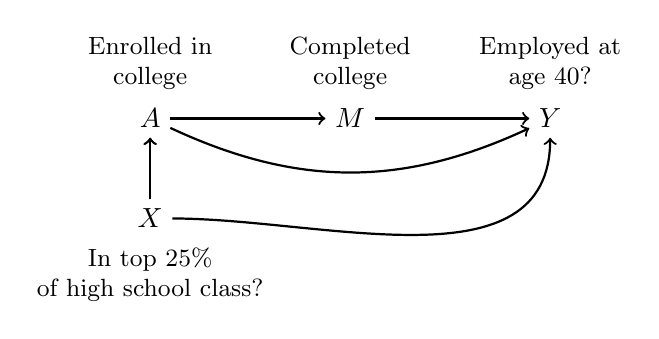
\begin{tikzpicture}[x = .5in, y = .5in]
    \node (x) at (-2,-1) {$X$};
    \node (a) at (-2,0) {$A$};
    \node (m) at (0,0) {$M$};
    \node (y) at (2,0) {$Y$};
    \draw[->, thick] (x) -- (a);
    \draw[->, thick] (a) to[bend right = 25] (y);
    \draw[->, thick] (a) -- (m);
    \draw[->, thick] (m) -- (y);
    \draw[->, thick] (x) -- (a);
    \draw[->, thick] (x) to[out = 0, in = 270] (y);
        % Labels
    \node[anchor = north, font = \small, align = center] at (x.south) {In top 25\%\\of high school class?};
    \node[anchor = south, font = \small, align = center] at (a.north) {Enrolled in\\college};
    \node[anchor = south, font = \small, align = center] at (m.north) {Completed\\college};
    \node[anchor = south, font = \small, align = center] at (y.north) {Employed at\\age 40?};
  \end{tikzpicture}
\end{center}
\pause
What three paths connect $A$ and $Y$? \\
Which two are causal paths? \vskip .1in
\pause
\begin{tabular}{ll}
$A\rightarrow Y$ & \only<5->{causal path} \\
$A\rightarrow M \rightarrow Y$ & \only<6->{causal path} \\
$A\leftarrow X \rightarrow Y$ & \only<7->{not a causal path}
\end{tabular}

\end{frame}

\begin{frame}[t]{Causal path: Marginal dependence}{$\bullet\rightarrow\bullet\rightarrow\bullet$} \vskip .2in

A causal path $A\rightarrow\cdots\rightarrow B$ will make the variables $A$ and $B$ statistically dependent \vskip .2in

Example:
$$(\text{visits grocery store}) \rightarrow (\text{buys ice cream}) \rightarrow (\text{eats ice cream})$$ \vskip .2in \pause

What if we condition:\\filter to those with (buys ice cream = \texttt{FALSE})?

\end{frame}

\begin{frame}[t]{Causal path: Conditional independence}{$\bullet\rightarrow\bullet\rightarrow\bullet$} \vskip .2in

A causal path $A\rightarrow\cdots\rightarrow B$ will not make the variables $A$ and $B$ statistically dependent if we condition on a variable along the path \vskip .2in

Example:
$$(\text{visits grocery store}) \rightarrow \boxed{(\text{buys ice cream})} \rightarrow (\text{eats ice cream})$$ \pause

Among people who didn't buy ice cream today,\\
those who went to the store and didn't\\
are equally likely to be eating ice cream. \vskip .2in \pause
Conditioning on (buys ice cream = \texttt{FALSE}) \textbf{blocks} this path.

\end{frame}

\subsection{Forks}

\begin{frame}[t]{Fork structure}{$\bullet\leftarrow\bullet\rightarrow\bullet$}

A sequence of edges within a path in which two variables are both caused by a third variable: $A\leftarrow C \rightarrow B$ \pause \vskip .1in

In our initial graph, what path contains a fork structure?

\begin{center}
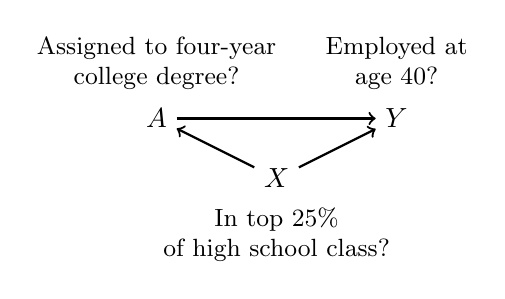
\begin{tikzpicture}[x = .3in, y = .3in]
    \node at (-3,0) {};
    \node at (3,0) {};
    \node (x) at (0,-1) {$X$};
    \node (a) at (-2,0) {$A$};
    \node (y) at (2,0) {$Y$};
    \draw[->, thick] (x) -- (a);
    \draw[->, thick] (a) -- (y);
    \draw[->, thick] (x) -- (y);
        % Labels
    \node[anchor = north, font = \small, align = center] at (x.south) {In top 25\%\\of high school class?};
    \node[anchor = south, font = \small, align = center] at (a.north) {Assigned to four-year\\college degree?};
    \node[anchor = south, font = \small, align = center] at (y.north) {Employed at\\age 40?};
  \end{tikzpicture}
\end{center}

Recall that there are two paths:
\begin{enumerate}
\item $A\rightarrow Y$
\item $A\leftarrow X \rightarrow Y$ \onslide<3->{(this path contains a fork structure)}
\end{enumerate}

\end{frame}

\begin{frame}[t]{Fork structure: Marginal dependence}{$\bullet\leftarrow\bullet\rightarrow\bullet$}

A fork structure $A\leftarrow C \rightarrow B$ will make $A$ and $B$ statistically dependent (because $C$ causes both). \vskip .1in

Example:
$$(\text{completed college}) \leftarrow (\text{top 25\% of high school})\rightarrow (\text{employed at 40})$$

\end{frame}

\begin{frame}[t]{Fork structure: Marginal dependence}{$\bullet\leftarrow\bullet\rightarrow\bullet$}

A fork structure $A\leftarrow C \rightarrow B$ will make $A$ and $B$ statistically dependent (because $C$ causes both). \vskip .1in

Example:
$$(\text{lifeguard rescues}) \leftarrow (\text{temperature})\rightarrow (\text{ice cream sales})$$ \pause

On days with many lifeguard rescues,\\there are also many ice cream sales.\\Warm temperature causes both. \vskip .2in \pause
What if we look only at days with a given temperature?

\end{frame}

\begin{frame}{Fork structure: Conditional independence}{$\bullet\leftarrow\bullet\rightarrow\bullet$}

A fork structure $A\leftarrow \boxed{C} \rightarrow B$ does not make $A$ and $B$ statistically dependent if we condition on $C$. \vskip .1in

Example:
$$(\text{lifeguard rescues}) \leftarrow \boxed{(\text{temperature})} \rightarrow (\text{ice cream sales})$$
Among days with a given temperature,\\lifeguard rescues and ice cream sales are unrelated. \vskip .2in
Conditioning on (temperature) blocks this path.

\end{frame}

\subsection{Colliders}

\begin{frame}{Collider structure}{$\bullet\rightarrow\bullet\leftarrow\bullet$}

A sequence of edges within a path in which two variables both cause a third variable: $A\rightarrow C \leftarrow B$ \pause \vskip .1in
Example:
\begin{itemize}
\item sprinklers on a timer
\item rain on random days
\item either one can make the grass wet
\end{itemize}

$$
(\text{sprinklers on}) \rightarrow (\text{grass wet}) \leftarrow (\text{raining})
$$ \pause
Are (sprinklers on) and (raining) statistically related?

\end{frame}

\begin{frame}{Collider structure: Marginal independence}{$\bullet\rightarrow\bullet\leftarrow\bullet$}

In a collider structure $A\rightarrow C \leftarrow B$,\\
$A$ and $B$ are marginally independent.
$$
(\text{sprinklers on}) \rightarrow (\text{grass wet}) \leftarrow (\text{raining})
$$
Knowing (sprinklers on = \texttt{TRUE}) tells me nothing about whether (raining = \texttt{TRUE}) \vskip .2in \pause

What if I condition: look only at days when the grass is wet?

\end{frame}

\begin{frame}{Collider structure: Conditional dependence}{$\bullet\rightarrow\bullet\leftarrow\bullet$}

$$
(\text{sprinklers on}) \rightarrow \boxed{(\text{grass wet})} \leftarrow (\text{raining})
$$ \vskip .2in \pause
Among days when (grass wet = \texttt{TRUE}),\\
if (sprinklers on = \texttt{FALSE})\\
then it must be (raining = \texttt{TRUE}) \vskip .1in
(grass had to get wet somehow!) \vskip .2in \pause

In a collider structure $A\rightarrow \boxed{C} \leftarrow B$,\\
$A$ and $B$ are conditionally dependent.

\end{frame}

\begin{frame}{Review: Three structures}

\begin{tabular}{llll}
& & $A$ and $B$ & $A$ and $B$ \\
& & marginally & conditionally \\
Name & Structure & dependent? & dependent given $C$? \\
\hline
Causal path & $A\rightarrow C \rightarrow B$ & Yes & No \\
Fork & $A\leftarrow C \rightarrow B$ & Yes & No \\
Collider & $A \rightarrow C \leftarrow B$ & No & Yes \\
\hline
\end{tabular}

\end{frame}

\subsection{Blocked Paths}

\begin{frame}[t]{A path can involve forks, colliders, and causal paths}

\begin{footnotesize}
$$
(\text{timer displays clock}) \leftarrow (\text{timer works}) \rightarrow (\text{sprinklers on}) \rightarrow (\text{grass wet}) \leftarrow (\text{raining})
$$
\end{footnotesize} \pause

(timer displays clock) is statistically related to which variables? \vskip .05in

\begin{tabular}{ll}
timer works & \onslide<3->{yes} \\
sprinklers on & \onslide<4->{yes} \\
grass wet & \onslide<5->{yes} \\
raining & \onslide<6->{no} \\
\end{tabular} \vskip .2in

\onslide<7->{We just learned: One collider can block an entire path}

\end{frame}

\begin{frame}[t]{A path can involve forks, colliders, and causal paths}

\begin{footnotesize}
$$
(\text{timer displays clock}) \leftarrow (\text{timer works}) \rightarrow \boxed{(\text{sprinklers on})} \rightarrow (\text{grass wet}) \leftarrow (\text{raining})
$$
\end{footnotesize} \pause

(timer displays clock) is statistically related to which variables? \vskip .05in

\begin{tabular}{ll}
timer works & \onslide<3->{yes} \\
grass wet & \onslide<4->{no} \\
raining & \onslide<5->{no} \\
\end{tabular} \vskip .2in

\onslide<6->{We just learned: One conditioned non-collider can block an entire path}

\end{frame}

\begin{frame}{Rules for whether paths are open or blocked}

\begin{itemize}
\item If a path contains an unconditioned collider, it is blocked
\item If a path contains a conditioned non-collider, it is blocked
\item Otherwise, the path is open
\end{itemize} \vskip .1in

Open paths create statistical dependence.\\Blocked paths do not.

\end{frame}

\subsection{Statistical Dependence}

\begin{frame}{Determining statistical dependence: A procedure}

How do you know if two nodes (e.g., $A$ and $B$ are dependent? \pause
\begin{center}
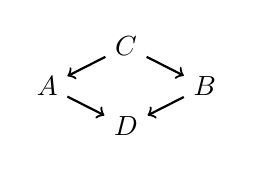
\begin{tikzpicture}[y = .2in]
\node (a) at (0,0) {$A$};
\node (b) at (2,0) {$B$};
\node (c) at (1,1) {$C$};
\node (d) at (1,-1) {$D$};
\draw[->, thick] (c) -- (a);
\draw[->, thick] (c) -- (b);
\draw[->, thick] (a) -- (d);
\draw[->, thick] (b) -- (d);
\end{tikzpicture}
\end{center} \pause
\begin{enumerate}
\item List all paths between the two nodes
\begin{itemize}
\item $A\leftarrow C \rightarrow B$
\item $A\rightarrow D \leftarrow B$
\end{itemize} \pause
\item Cross out any blocked paths that are blocked
\begin{itemize}
\item $A\leftarrow C \rightarrow B$
\item \st{$A\rightarrow D \leftarrow B$}
\end{itemize} \pause
\item If any paths remain, the two nodes are dependent
\begin{itemize}
\item Dependent!
\end{itemize}
\end{enumerate}

\end{frame}

% BUILDING UP EXAMPLE

\begin{frame}[t]{Determining statistical dependence: A procedure}{1. List all paths. 2. Cross out blocked paths. 3. Dependent if any paths remain.} \pause
\begin{center}
  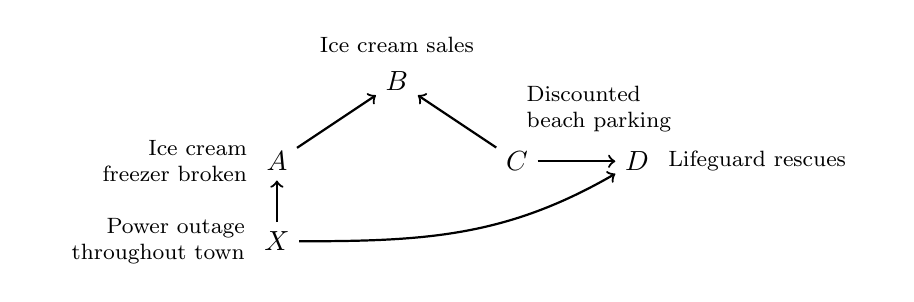
\begin{tikzpicture}[x = .6in, y = .4in]
  \node at (-2,0) {};
  \node at (5,0) {};
  \node (x) at (0,-1) {$X$};
  \node[anchor = east, font = \footnotesize, align = right] at (x.west) {Power outage\\throughout town};
  \pause
  \node (a) at (0,0) {$A$};
  \node[anchor = east, font = \footnotesize, align = right] at (a.west) {Ice cream\\freezer broken};
  \draw[->, thick] (x) -- (a);
  \pause
  \node (b) at (1,1) {$B$};
  \node[anchor = south, font = \footnotesize, align = right] at (b.north) {Ice cream sales};
  \draw[->, thick] (a) -- (b);
  \pause
  \node (c) at (2,0) {$C$};
  \node[anchor = south west, font = \footnotesize, align = left] at (c.north) {Discounted\\beach parking};
  \draw[->, thick] (c) -- (b);
  \pause
  \node (d) at (3,0) {$D$};
  \node[anchor = west, font = \footnotesize, align = right] at (d.east) {Lifeguard rescues};
  \draw[->, thick] (c) -- (d);
  \pause
  \draw[->, thick] (x) to[out = 0, in = 210] (d);
  \end{tikzpicture}
\end{center}
\end{frame}

% MARGINAL A AND C
\begin{frame}[t]{Determining statistical dependence: A procedure}{1. List all paths. 2. Cross out blocked paths. 3. Dependent if any paths remain.}
\begin{center}
  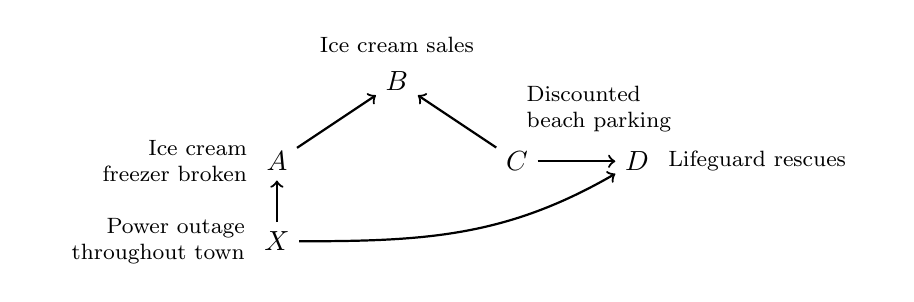
\begin{tikzpicture}[x = .6in, y = .4in]
  \node at (-2,0) {};
  \node at (5,0) {};
  \node (x) at (0,-1) {$X$};
  \node (a) at (0,0) {$A$};
  \node (b) at (1,1) {$B$};
  \node (c) at (2,0) {$C$};
  \node (d) at (3,0) {$D$};
  \draw[->, thick] (a) -- (b);
  \draw[->, thick] (c) -- (b);
  \draw[->, thick] (c) -- (d);
  \draw[->, thick] (x) -- (a);
  \draw[->, thick] (x) to[out = 0, in = 210] (d);
  \node[anchor = east, font = \footnotesize, align = right] at (a.west) {Ice cream\\freezer broken};
  \node[anchor = east, font = \footnotesize, align = right] at (x.west) {Power outage\\throughout town};
  \node[anchor = south, font = \footnotesize, align = right] at (b.north) {Ice cream sales};
  \node[anchor = south west, font = \footnotesize, align = left] at (c.north) {Discounted\\beach parking};
  \node[anchor = west, font = \footnotesize, align = right] at (d.east) {Lifeguard rescues};
  \end{tikzpicture}
\end{center}
Are $A$ and $C$ statistically independent or dependent?
\pause
\begin{itemize}
\item \only<3->{\st}{$A\rightarrow B \leftarrow C$}
\item \only<4->{\st}{$A\leftarrow X \rightarrow D \leftarrow C$}
\end{itemize}
\only<5>{No unblocked paths. Independent!}
\end{frame}

% MARGINAL A AND D
\begin{frame}[t]{Determining statistical dependence: A procedure}{1. List all paths. 2. Cross out blocked paths. 3. Dependent if any paths remain.}
\begin{center}
  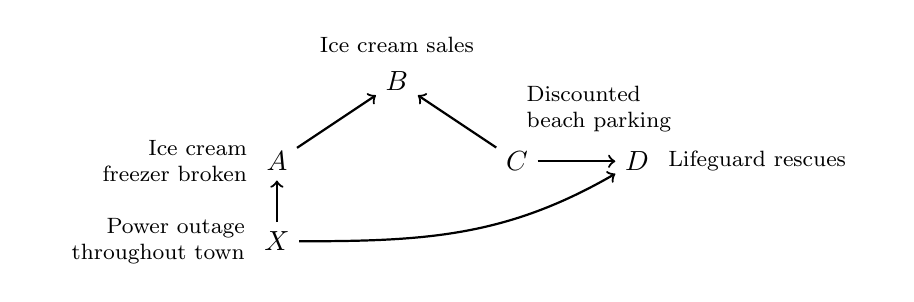
\begin{tikzpicture}[x = .6in, y = .4in]
  \node at (-2,0) {};
  \node at (5,0) {};
  \node (x) at (0,-1) {$X$};
  \node (a) at (0,0) {$A$};
  \node (b) at (1,1) {$B$};
  \node (c) at (2,0) {$C$};
  \node (d) at (3,0) {$D$};
  \draw[->, thick] (a) -- (b);
  \draw[->, thick] (c) -- (b);
  \draw[->, thick] (c) -- (d);
  \draw[->, thick] (x) -- (a);
  \draw[->, thick] (x) to[out = 0, in = 210] (d);
  \node[anchor = east, font = \footnotesize, align = right] at (a.west) {Ice cream\\freezer broken};
  \node[anchor = east, font = \footnotesize, align = right] at (x.west) {Power outage\\throughout town};
  \node[anchor = south, font = \footnotesize, align = right] at (b.north) {Ice cream sales};
  \node[anchor = south west, font = \footnotesize, align = left] at (c.north) {Discounted\\beach parking};
  \node[anchor = west, font = \footnotesize, align = right] at (d.east) {Lifeguard rescues};
  \end{tikzpicture}
\end{center}
Are $A$ and $D$ statistically independent or dependent? \pause
\begin{itemize}
\item \only<3->{\st}{$A\rightarrow B \leftarrow C \rightarrow D$}
\item $A\leftarrow X \rightarrow D$
\end{itemize}
\only<4>{A path remains unblocked. Dependent!}

\end{frame}

% CONDITIONAL

%\section{Conditional Dependence}

\begin{frame}

\huge
Practice with \textbf{conditional} dependence\\
(holding something constant)

\end{frame}

\begin{frame}[t]{Determining statistical dependence: A procedure}{1. List all paths. 2. Cross out blocked paths. 3. Dependent if any paths remain.}
\begin{center}
  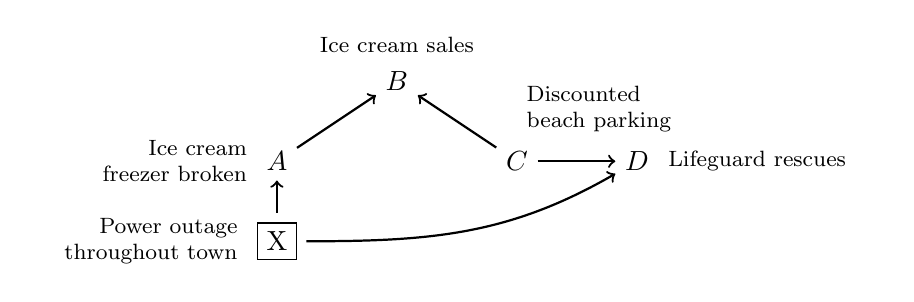
\begin{tikzpicture}[x = .6in, y = .4in]
  \node at (-2,0) {};
  \node at (5,0) {};
  \node (x) at (0,-1) {\boxed{$X$}};
  \node (a) at (0,0) {$A$};
  \node (b) at (1,1) {$B$};
  \node (c) at (2,0) {$C$};
  \node (d) at (3,0) {$D$};
  \draw[->, thick] (a) -- (b);
  \draw[->, thick] (c) -- (b);
  \draw[->, thick] (c) -- (d);
  \draw[->, thick] (x) -- (a);
  \draw[->, thick] (x) to[out = 0, in = 210] (d);
  \node[anchor = east, font = \footnotesize, align = right] at (a.west) {Ice cream\\freezer broken};
  \node[anchor = east, font = \footnotesize, align = right] at (x.west) {Power outage\\throughout town};
  \node[anchor = south, font = \footnotesize, align = right] at (b.north) {Ice cream sales};
  \node[anchor = south west, font = \footnotesize, align = left] at (c.north) {Discounted\\beach parking};
  \node[anchor = west, font = \footnotesize, align = right] at (d.east) {Lifeguard rescues};
  \end{tikzpicture}
\end{center}
Practice: Are $A$ and $D$ statistically independent or dependent, conditional on $X = \texttt{FALSE}$?
\pause
  \begin{itemize}
\item \only<3->{\st}{$A\rightarrow B \leftarrow C \rightarrow D$}
\item \only<4->{\st}{$A\leftarrow \boxed{X} \rightarrow D$}
\end{itemize}
\only<5>{No unblocked paths. Independent!}
\end{frame}
  
\begin{frame}[t]{Determining statistical dependence: A procedure}{1. List all paths. 2. Cross out blocked paths. 3. Dependent if any paths remain.}
\begin{center}
  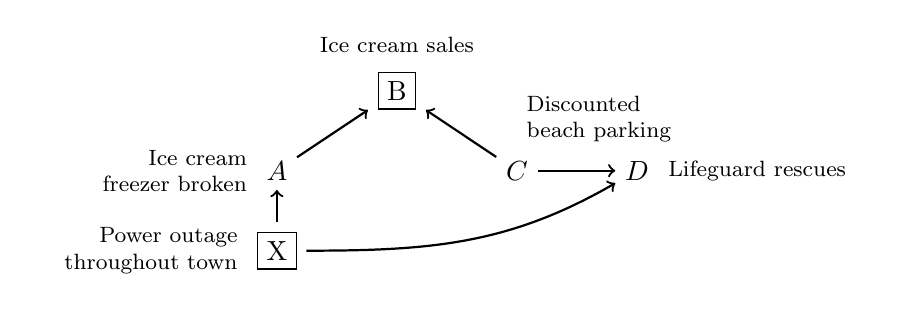
\begin{tikzpicture}[x = .6in, y = .4in]
  \node at (-2,0) {};
  \node at (5,0) {};
  \node (x) at (0,-1) {\boxed{$X$}};
  \node (a) at (0,0) {$A$};
  \node (b) at (1,1) {\boxed{$B$}};
  \node (c) at (2,0) {$C$};
  \node (d) at (3,0) {$D$};
  \draw[->, thick] (a) -- (b);
  \draw[->, thick] (c) -- (b);
  \draw[->, thick] (c) -- (d);
  \draw[->, thick] (x) -- (a);
  \draw[->, thick] (x) to[out = 0, in = 210] (d);
  \node[anchor = east, font = \footnotesize, align = right] at (a.west) {Ice cream\\freezer broken};
  \node[anchor = east, font = \footnotesize, align = right] at (x.west) {Power outage\\throughout town};
  \node[anchor = south, font = \footnotesize, align = right] at (b.north) {Ice cream sales};
  \node[anchor = south west, font = \footnotesize, align = left] at (c.north) {Discounted\\beach parking};
  \node[anchor = west, font = \footnotesize, align = right] at (d.east) {Lifeguard rescues};
  \end{tikzpicture}
\end{center}
Practice: Are $A$ and $D$ statistically independent or dependent, conditional on $X = \texttt{FALSE}$ and $B = \texttt{0}$?
\pause
  \begin{itemize}
\item $A\rightarrow \boxed{B} \leftarrow C \rightarrow D$
\item \only<3->{\st}{$A\leftarrow \boxed{X} \rightarrow D$}
\end{itemize}
\only<4>{A path remains. Dependent!}
\end{frame}

\begin{frame}{DAGs and conditional exchangeability}

When studying the effect of $A$ on $Y$, conditional exchangeability holds if the only unblocked paths between $A$ and $Y$ are causal paths from $A$ to $Y$. \pause
\begin{itemize}
\item Why? Because then any association between $A$ and $Y$ must be due to the causal effect
\end{itemize} \pause
\begin{center}
  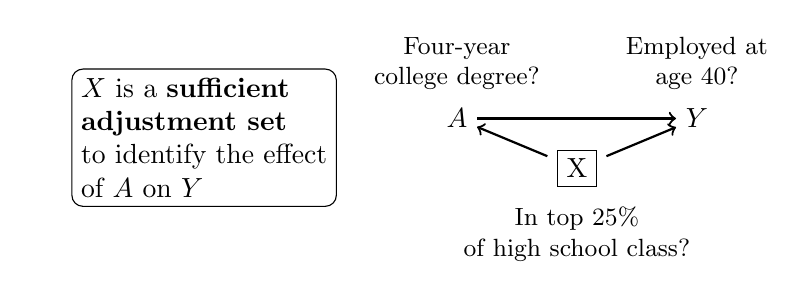
\begin{tikzpicture}[x = .3in, y = .25in]
    \node at (-9,0) {};
    \node at (3,0) {};
    \node (x) at (0,-1) {\boxed{$X$}};
    \node (a) at (-2,0) {$A$};
    \node (y) at (2,0) {$Y$};
    \draw[->, thick] (x) -- (a);
    \draw[->, thick] (a) -- (y);
    \draw[->, thick] (x) -- (y);
    % Labels
    \node[anchor = north, font = \small, align = center] at (x.south) {In top 25\%\\of high school class?};
    \node[anchor = south, font = \small, align = center] at (a.north) {Four-year\\college degree?};
    \node[anchor = south, font = \small, align = center] at (y.north) {Employed at\\age 40?};
    \node<5->[anchor = north east, align = left, draw, rounded corners] at (-4,1) {$X$ is a \textbf{sufficient}\\\textbf{adjustment set}\\to identify the effect\\of $A$ on $Y$};
  \end{tikzpicture}
  \end{center} \pause
\begin{itemize}
\item $A\rightarrow Y$
\item $A\leftarrow \boxed{X} \rightarrow Y$ (blocked by conditioning on $X$)
\end{itemize}

\end{frame}

\begin{frame}{DAGs and conditional exchangeability: Practice}
{1. List all paths. 2. Choose adjustment set. 3. Only causal paths remain unblocked.}

\begin{center}
  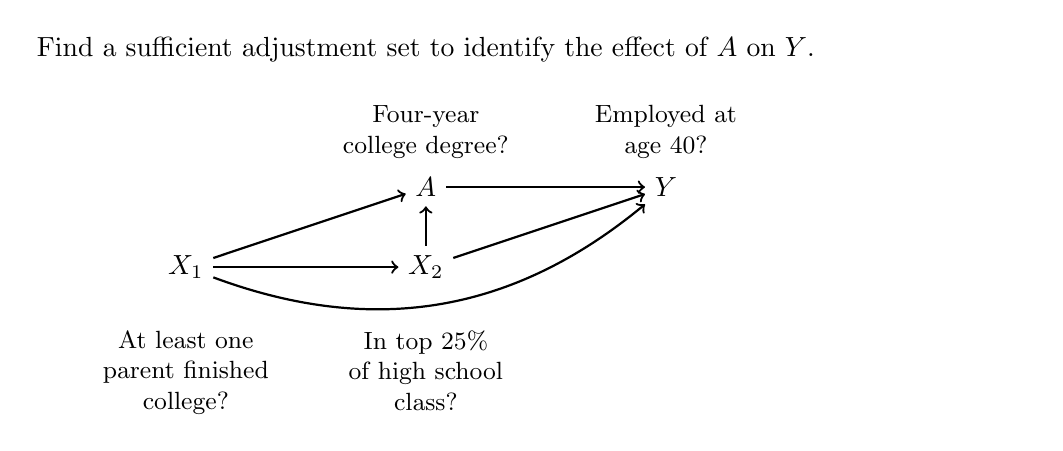
\begin{tikzpicture}[x = .6in, y = .4in]
  \node[anchor = north] at (-2,2) {Find a sufficient adjustment set to identify the effect of $A$ on $Y$.};
    \node at (-3,0) {};
    \node at (3,0) {};
    \node (x1) at (-4,-1) {$X_1$};
    \node (x2) at (-2,-1) {$X_2$};
    \node (a) at (-2,0) {$A$};
    \node (y) at (0,0) {$Y$};
    \draw[->, thick] (x1) -- (a);
    \draw[->, thick] (x1) to[bend right = 30] (y);
    \draw[->, thick] (x1) -- (x2);
    \draw[->, thick] (x2) -- (a);
    \draw[->, thick] (a) -- (y);
    \draw[->, thick] (x2) -- (y);
    % Labels
    \node[anchor = north, font = \small, align = center, outer sep = 12pt] at (x1.south) {At least one\\parent finished\\college?};
    \node[anchor = north, font = \small, align = center, outer sep = 12pt] at (x2.south) {In top 25\%\\of high school\\class?};
    \node[anchor = south, font = \small, align = center] at (a.north) {Four-year\\college degree?};
    \node[anchor = south, font = \small, align = center] at (y.north) {Employed at\\age 40?};
  \end{tikzpicture}
  \end{center} \pause

Paths: ($A\rightarrow Y$), ($A\leftarrow X_2\rightarrow Y$), ($A\leftarrow X_1\rightarrow Y$), ($A\leftarrow X_1\rightarrow X_2\rightarrow Y$),($A\leftarrow X_2\leftarrow X_1\rightarrow Y$) \\ \pause
Adjust for \{$X_1,X_2\}$

\end{frame}

\begin{frame}{How to draw a DAG}

\begin{enumerate}
\item Begin with treatment $A$ and outcome $Y$
\item Add any variable that affects both
\item Add any variable that affects any two variables in the DAG.
\end{enumerate}

Assumptions are about nodes and edges that you omit.

\end{frame}

\begin{frame}{Exercise: Draw a DAG}

Treatment is college degree. Outcome is employment at age 40. \\
Identify a sufficient adjustment set under your DAG.

\end{frame}

\goalsframe

\end{document}
